\chapter{Certification Methods for Adversarial Examples}
\minitoc
\label{chap:certification}
In this chapter we focus on noise injection and convex flows to build certifiable defenses on adversarial robustness. A desirable property for a function to be robust against adversarial examples is that the classifier $\mathbf{f}=(f_1,\dots,f_K)$ is a $M$-Lipschitz function with regards to Euclidean norm i.e. $\lVert \mathbf{f}(x)-\mathbf{f}(x')\rVert_2\leq M\lVert x-x'\rVert$ for all $x,x'\in\mathcal{X}$. 

\begin{prop}[\citep{li2019preventing}]Let $\mathbf{f}$ be a  $M$-Lipschitz classifier. Then for $\varepsilon>0$ and for every $x$ with label $y$ such that \begin{align*}
    \max(0,f_y(x)-\max_{y'\neq y}f_{y'}(x))> \sqrt{2}M\varepsilon
\end{align*}
then we have for every $\tau$ such that $\lVert \tau\rVert\leq \varepsilon$:
\begin{align*}
    \argmaxB_{i}f_i(x+\tau)=y
\end{align*}
\end{prop}

This property ensures robustness guarantees for Lipschitz classifiers


\section{Certification using Noise Injection}
As we will inject some noise in our classifier in order to defend against adversarial attacks, we need to introduce the notion of ``probabilistic mapping''.

\begin{definition}[Probabilistic mapping] Let $\mathcal{X}$ be an arbitrary space, and $(\mathcal{Y},\mathcal{F}_{\mathcal{Y}})$ a measurable space. A \emph{probabilistic mapping} from $\mathcal{X}$ to $\mathcal{Y}$ is a randomized classifier, i.e. a mapping $\probmap: \mathcal{X} \to \mathcal{M}_1^+(\mathcal{Y})$.
To obtain a numerical output out of this \emph{probabilistic mapping}, one needs to sample $y$ according to $\probmap(x)$. %$y\sim \probmap(x)$.
\end{definition} 

Any mapping can be considered as a probabilistic mapping, whether it explicitly injects noise (as in~\citep{lecuyer2018certified,rakin2018parametricnoiseinjection,pruningDefenseICLR2018}) or not. In fact, any deterministic mapping can be considered as a probabilistic mapping, since it can be characterized by a Dirac measure. Accordingly, the definition of a probabilistic mapping is fully general and equally treats networks with or without noise injection. There exists no definition of robustness against adversarial attacks that comply with the notion of probabilistic mappings. We settle that by generalizing the notion of prediction-change risk initially introduced in~\citep{NIPS2018Mahloujifar} for deterministic classifiers. Let $\probmap$ be a probabilistic mapping from $\mathcal{X}$ to $\mathcal{Y}$, and $d_{\mathcal{M}_1^+(\mathcal{Y})}$ some metric/divergence on $\mathcal{M}_1^+(\mathcal{Y})$. We define the $(\varepsilon,\alpha)$-radius prediction-change risk of $\probmap$ w.r.t. $\mathcal{D}_{\mathcal{X}}$ and $d_{\mathcal{M}_1^+(\mathcal{Y})}$ as 
$$\PCadvRisk(\probmap,\alpha):=  \mathbb{P}_{x\sim \mathcal{D}_{\mathcal{X}}}\left[ \exists \tau \in B(\varepsilon) \text{ s.t. } d_{\mathcal{M}_1^+(\mathcal{Y})}(\probmap(x+\tau),\probmap(x)) > \alpha \right] \enspace.$$

These three generalized notions allow us to analyze noise injection defense mechanisms (Theorems~\ref{thm:netrob}, and~\ref{thm:bound}). We can also define adversarial robustness (and later adversarial gap) thanks to these notions. 

\begin{definition}[Adversarial robustness]
\label{def::GeneralizedRobustness}
Let $d_{\mathcal{M}_1^+(\mathcal{Y})}$ be a metric/divergence on $\mathcal{M}_1^+(\mathcal{Y})$. A probabilistic mapping $\probmap$ is called
 $d_{\mathcal{M}_1^+(\mathcal{Y})}$-$(\varepsilon, \alpha, \gamma)$ robust if
$\PCadvRisk(\probmap,\alpha) \leq \gamma$, $d_{\mathcal{M}_1^+(\mathcal{Y})}$-$(\varepsilon, \alpha)$ robust if $\gamma = 0$.
\end{definition}

% \begin{definition}[Adversarial gap]
% \label{def::adversarialgap}
% Let $\probmap$ be a probabilistic mapping from $\mathcal{X}$ to $\mathcal{Y}$. The $\varepsilon$-radius adversarial gap of $\probmap$ is defined as $\text{Gap}_{\varepsilon}(\probmap) = |\advRisk(K) - \Risk(K)|$
% \end{definition}

It is difficult in general to show that a classifier is $d_{\mathcal{M}_1^+(\mathcal{Y})}$-$(\varepsilon, \alpha, \gamma)$ robust. However, we can  derive some bounds for particular divergences that will ensure robustness up to a certain level (Theorem~\ref{thm:netrob}). It is worth noting that our definition of robustness depends
on the considered metric/divergence between probability measures. Lemma~\ref{th::PropimpliesRobustness} gives some insights on the monotony of the robustness according to the parameters, and the probability metric/divergence at hand.

% One needs to be careful when considering adversarial robustness regarding this definition: a robust mapping does not necessarily ensures accuracy. In fact, if $\mathcal{Y}$ is the space of labels $\left[N\right ]$ and $u(x+\tau),u(x)$ respect the same uniform distribution over $\mathcal{Y}$, then for every metric/divergence $d$, one has $d(u(x+\tau),u(x))=0$, and the accuracy will be the one of a random classifier. In the following, \textit{robust} will mean robust in the sense of Definition~\ref{def::GeneralizedRobustness}. Our definition depends on $3$ parameters ($\varepsilon$,$\alpha$,$\gamma$) and on the metric/divergence one chooses to consider between probability measures. Lemma~\ref{th::PropimpliesRobustness} gives some natural insights on the monotony of the robustness according to the parameters, and the probability metric at hand.






%\section{Using Exponential family for adversarial robustness}

%In the following of the paper, we will consider a measurable metric input space $\mathcal{X}$. We denote $\norm{.}_{\mathcal{X}}$ a norm on $\mathcal{X}$ and we suppose the inputs are samples from a distribution $\mathcal{D}$. 




%\subsection{Adversarial attacks problem}
%Let us consider a classification task\footnote{Note that the definition of robustness we provide generalizes to other tasks.} over $\mathcal{X}$. A data $x\in\mathcal{X}$ has a true label $y_{true}\in \left [ N\right ]$. Let  $\hat{f}$ be a trained classifier over $\mathcal{X}$. The problem of generating an adversarial example from an input $x$ writes:

%where $t$ is the target class (with $t\neq \hat{f}(x)$).
%Equation (\ref{attackclassicalproblem}) presents a targeted attack model. For the untargeted attack problem, the condition is changed from $\hat{f}(x+\tau)=t$ to $\hat{f}(x+\tau)\neq \hat{f}(x)$. In this paper, we treat indifferently targeted and untargeted attacks. Figure~\ref{advattack} illustrates the principle of an adversarial attack on $\hat{f}$: a small perturbation $\tau$ applied on an input $x$ fools the classifier. The dashed line represents the boundary decision between two classes. The dashed circle around $x$ represents the maximal amount of noise keeping the adversarial example perceptually close to $x$ (in the case of images). The inputs $x$ and $x+\tau$ looks similar but they are classified with two different labels.


%\begin{figure}[ht]
%\vskip 0.2in
%\begin{center}
%\centerline{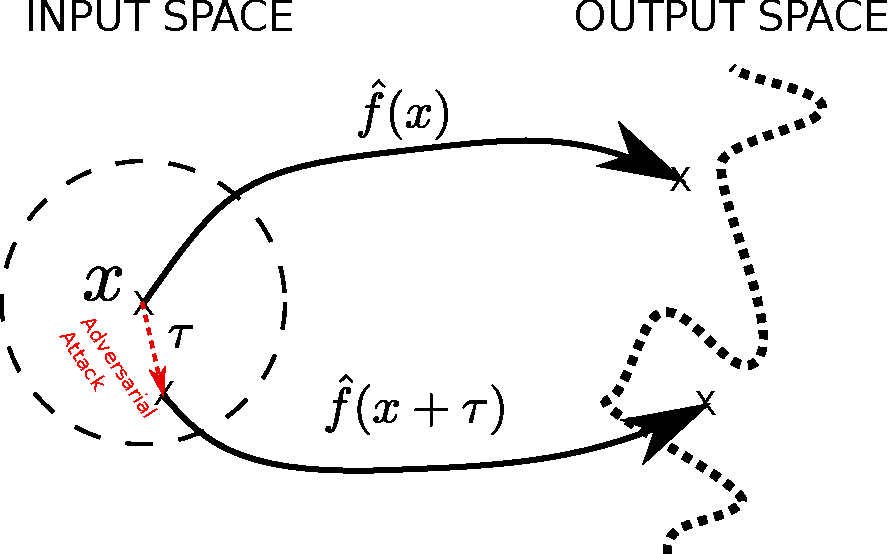
\includegraphics[width=0.5\columnwidth]{images/advAttackV5.pdf}}
%\caption{Illustration of an adversarial attack on a classifier $\hat{f}$. } 
%\label{advattack}
%\end{center}
%\vskip -0.2in
%\end{figure}



%\subsection{A general definition of robustness to adversarial attacks}
%\label{subsec:def}

%As we will inject noise in our algorithm in order to defend against adversarial attacks, we need to introduce the notion of ``probabilistic mapping''. Let us consider $\mathcal{Y}$ the output space, and $\mathcal{F}_{\mathcal{Y}}}$ a $\sigma$-$ algebra$ over $\mathcal{Y}$.

%\begin{definition}[Probabilistic mapping] Let $(\mathcal{Y},\mathcal{F}_{\mathcal{Y}}})$ be a measurable space. For any space $\mathcal{X}$, a \emph{probabilistic mapping} from $\mathcal{X}$ to $\mathcal{Y}$ is a mapping $u: \mathcal{X} \to \mathcal{M}_1^+(\mathcal{Y})$ where $\mathcal{M}_1^+(\mathcal{Y})$ is the set of probability measures over $(\mathcal{Y},\mathcal{F}_{\mathcal{Y}}})$.
%To obtain a numerical output out of this mechanism, one needs to sample $y\sim u(x)$.
%\end{definition} 

% This definition does not depend on the nature of $\mathcal{Y}$ as long as $(\mathcal{Y},\mathcal{F}_{\mathcal{Y}}})$ is measurable. In that sense, $\mathcal{Y}$ could be either the label space $\left[N\right]$ or any  intermediate space corresponding to the outputs of one hidden layer of a neural network. Moreover, any mapping can be considered as a probabilistic mapping, whether it explicitly injects noise (as in~\citep{lecuyer2018certified,rakin2018parametricnoiseinjection,pruningDefenseICLR2018}) or not. In fact, any deterministic mapping can be considered as a probabilistic mapping, since it can be characterized by a Dirac measure. Accordingly, the definition of a probabilistic mapping is fully general and equally treats networks with or without noise injection. So far, there exists no definition of robustness against adversarial attacks that comply with the notion of probabilistic mappings.  We settle that by generalizing the notion of prediction-change risk initially introduced in~\citep{NIPS2018Mahloujifar} for deterministic classifiers. Given a classifier $h$ it is defined as follows:
% $$Risk_\varepsilon(h)= \mathbb{P}_{x\sim \mathcal{D}}\left[ \exists \tau \in B(\varepsilon) \text{ s.t.} h(x+\tau)\neq h(x) \right] $$
% where for any $\varepsilon \geq 0$, $B(\varepsilon) =\{\tau \in \mathcal{X} \text{ s.t.} \norm{\tau}_{\mathcal{X}} \leq \varepsilon \}$. 

% In our case, as probabilistic mappings are considered, we need to generalize this notion to probability measures. This leads to the following definition.
% %Literature on robustness against adversarial examples attacks mostly focuses on the classification setting. Therefore, this work presents a classification task. Our framework could yet adapt to regression, or any other task.



% \begin{definition}[Adversarial robustness]
% \label{def::GeneralizedRobustness}
% Let $d_{\mathcal{M}_1^+(\mathcal{Y})}$ be a metric/divergence on $\mathcal{M}_1^+(\mathcal{Y})$. The probabilistic mapping $u$ is said to be $d_{\mathcal{M}_1^+(\mathcal{Y})}$-$(\varepsilon, \alpha, \gamma)$-robust if:
% $$\mathbb{P}_{x\sim \mathcal{D}}\left[ \exists \tau \in B(\varepsilon) \text{ s.t.} d_{\mathcal{M}_1^+(\mathcal{Y})}(u(x+\tau),u(x)) > \alpha \right] \leq \gamma. $$
% \end{definition}


% Finally, conversely to the previous work, ours does not restrict neither the task (regression, classification, reinforcement learning, etc.) nor the type of distribution the perturbation is drawn from. As $\mathcal{Y}$ is an arbitrary space, this notion of robustness for probabilistic mappings is fully general, but, in this paper, our final goal remains to ensure robustness for a classification task.
% Computing exact divergences and probability measures is unfeasible in practice because neural network functions are too much complicated. But, we can manage to obtain bounds pour divergences that will ensure robustness up to a certain level.

% One needs to be careful when considering adversarial robustness regarding this definition: a robust mapping does not necessarily ensures accuracy. In fact, if $\mathcal{Y}$ is the space of labels $\left[N\right ]$ and $u(x+\tau),u(x)$ respect the same uniform distribution over $\mathcal{Y}$, then for every metric/divergence $d$, one has $d(u(x+\tau),u(x))=0$, and the accuracy will be the one of a random classifier. In the following, \textit{robust} will mean robust in the sense of Definition~\ref{def::GeneralizedRobustness}. Our definition depends on $3$ parameters ($\varepsilon$,$\alpha$,$\gamma$) and on the metric/divergence one chooses to consider between probability measures. Lemma~\ref{th::PropimpliesRobustness} gives some natural insights on the monotony of the robustness according to the parameters, and the probability metric at hand.
% In particular one could consider the deterministic setting by fixing the considered probability measures as Dirac measures, $d_{\mathcal{M}_1^+(\mathcal{Y})}$ as the trivial distance, and $\alpha$ to $0$.
%  In practice, it might be quite hard to evaluate the probability from Definition~\ref{def::GeneralizedRobustness} for any given probabilistic mapping. Nevertheless, as presented in Section~\ref{section::noiseselection}, one should, and can produce algorithms that are robust by design with a noise drawn from an Exponential family.
 
 %In fact one doesn't have access to the ground-truth function, and thus is not able to evaluate $B(\varepsilon)$. Section~\ref{section::noiseselection} will give simple and efficient techniques to comply with the definition, while avoiding to compute this probability.
 


\begin{lemma}
\label{th::PropimpliesRobustness}Let $\probmap$ be a probabilistic mapping, and
let  $d_{1}$ and $d_{2}$ be two metrics on $\mathcal{M}_1^+(\mathcal{Y})$.
If there exists a non decreasing function $ \phi: \mathbb{R} \to \mathbb{R}$ such that  $\forall \mu_1,\mu_2 \in \mathcal{M}_1^+(\mathcal{Y})$, $d_{1}(\mu_1,\mu_2) \leq \phi(d_{2}(\mu_1,\mu_2)) $, then the following assertion holds: 
$\probmap \text{ is } d_{2}\text{-}(\varepsilon, \alpha, \gamma)\text{-robust} \implies \probmap \text{ is }d_{1}\text{-}(\varepsilon, \phi(\alpha), \gamma)\text{-robust}.$
\end{lemma}

As suggested in Definition~\ref{def::GeneralizedRobustness} and Lemma~\ref{th::PropimpliesRobustness}, any given choice of metric/divergence will instantiate a particular notion of adversarial robustness and it should be carefully selected. %The joint goals that should naturally lead to the selection of an appropriate metric/divergence are its coherence with the task at hand, and its strength (we define strength as being able to cover a wide number of other metrics regarding Lemma~\ref{th::PropimpliesRobustness}). 


% \subsubsection{On the choice of the metric/divergence for robustness}
% \label{subsec:div}
% % \Jam{This section needs to be re-organized and simplified. I argue for telling the whole story in a an 'hors d'oeuvre' paragraph before going deeper in the math. To discuss of course. The narration could be as follows, the divergence/metric that generalizes the Bayes risk is the trivial distance with is untractable, but hopefully there is another measure that is related to the Bayes risk is the total variance, which has good properties, however it is still untractable, an hopefully again we have a generalized divergence that provide a rich landscape of behaviors, this one is Renyi...But at the end what we are looking for is a good divergence with goof properties....}

% % \Lau{CHANGED}

% The aforementioned formulation naturally raises the question of the choice of the metric used to defend against adversarial attacks. 
% %At this point, a natural question to be asked is the choice of the metric/divergence we will choose to defend against adversarial attacks. 
% The main notions that govern the selection of an appropriate metric/divergence are  \emph{coherence}, \emph{strength}, and \emph{computational tractability}. A metric/divergence is said to be coherent if it naturally fits the task at hand ({\em e.g.} classification tasks are intrinsically linked to discrete/trivial metrics, conversely to regression tasks). The strength of a metric/divergence refers to its ability to cover (dominate) a wide class of others in the sense of Lemma~\ref{th::PropimpliesRobustness}. 
% In the following, we will focus on both the total variation metric and the Renyi divergence, that we consider as respectively the most coherent with the classification task using probabilistic mappings, and the strongest divergence. We first discuss how total variation metric is \emph{coherent} with randomized classifiers but suffers from computational issues. The Renyi divergence provides good guarantees about adversarial robustness, enjoys nice \emph{computational properties}, in particular when considering  Exponential family distributions, and is \emph{strong} enough to dominate a wide range of metrics/divergences including total variation.

% % \textbf{Dominated measure:} $\mu$ is said to be \emph{dominated} by $\nu$ (denoted $\mu \ll \nu$) if and only if for all $Y \in \mathcal{F}_{\mathcal{Y}}}$, $\ \nu(Y) = 0 \implies \mu(Y)=0$. If $\mu$ is dominated by $\nu$, there is a measurable function $h : \mathcal{Y} \rightarrow [0,+\infty)$ such that for all $Y \in \mathcal{F}_{\mathcal{Y}}}$, $ \mu(Y)=\int_{Y} h \ d\nu$. $ h $ is called the Radon-Nikodym derivative and is denoted $\frac{d \mu}{d \nu}$.

%  Let  $\mu_1$ and $\mu_2$ be two measures in $\mathcal{M}_1^+(\mathcal{Y})$, both dominated by a third measure $\nu$. The trivial distance $ d_{T}(\mu_1,\mu_2):= \mathds{1}\left(\mu_1 \neq \mu_2\right)$ is the simplest distance one can define between $\mu_1$ and $\mu_2$. In the deterministic case, it is straightforward to compute (since the numerical output of the algorithm characterizes its associated measure), but this is not the case in general. In fact one might not have access to the true distribution of the mapping, but just to the numerical outputs. Therefore, one needs to consider more sophisticated metrics/divergences, such as the total variation distance $ d_{TV}(\mu_1,\mu_2):= \sup_{Y \in \mathcal{F}_{\mathcal{Y}}} |\mu_1 (Y) - \mu_2(Y)|.$ The total variation distance is one of the most broadly used probability metrics. It admits several very simple interpretations, and is a very useful tool in many mathematical fields such as probability theory, Bayesian statistics, coupling or transportation theory. In transportation theory, it can be rewritten as the solution of the Monge-Kantorovich problem with the cost function $c(y_1,y_2) =\mathds{1}\left(y_1 \neq y_2\right)$:
% $ \inf\int_{\mathcal{Y}^{2}}\mathds{1}\left(y_1 \neq y_2\right) d\pi(y_1,y_2)\, ,$
% where the infimum is taken over all joint probability measures $\pi$ on $(\mathcal{Y}\times \mathcal{Y}, \mathcal{F}_{\mathcal{Y} } \otimes \mathcal{F}_{\mathcal{Y}})$ with marginals $\mu_1$ and $\mu_2$. According to this interpretation, it seems quite natural to consider the total variation distance as a relaxation of the trivial distance on $[0,1]$ (see~\citep{villani2003topics} for details). In the deterministic case, the total variation and the trivial distance coincides. In general, the total variation allows a finer analysis of the probabilistic mappings than the trivial distance. But it suffers from a high computational complexity. In the following of the paper we will show how to ensure robustness regarding TV distance.

% Finally, denoting by $g_1$ and $g_2$ the respective probability distributions w.r.t. $\nu$,  the Renyi divergence of order $\lambda$~\citep{renyi1961} writes as  $d_{R,\lambda}(\mu_1,\mu_2):=\frac{1}{\lambda -1}\log \int_{\mathcal{Y}} g_2(y)  \left(\frac{g_1(y)}{g_2(y)}\right)^{\lambda} d\nu(y).$
% The Renyi divergence is a generalized measure defined on the interval $(1,\infty)$, where it equals the Kullback-Leibler divergence when $\lambda \rightarrow 1$ (that will be denoted $d_{KL}$), and the maximum divergence when $\lambda \rightarrow \infty$. It also has the very special property of being non decreasing w.r.t. $\lambda$. This divergence is very common in machine learning, especially in its Kullback-Leibler form as it is widely used as the loss function (cross entropy) of classification algorithms. It enjoys the desired properties  since it bounds the TV distance, and is tractable.  Furthermore, Proposition~\ref{prop:RobustTV} proves that Renyi-robustness implies TV-robustness, making it a suitable surrogate for the trivial distance.

\begin{prop}[Renyi implies TV-robustness]
\label{prop:RobustTV}
Let $\probmap$ be a probabilistic mapping, then for all $\lambda\geq1$, $\alpha > 0$, there exists $\alpha' > 0$ s.t. if $\probmap \text{ is }  d_{R,\lambda}\text{-}(\varepsilon, \alpha, \gamma)\text{-robust}$ then $\probmap \text{ is } d_{TV}\text{-}(\varepsilon, \alpha', \gamma)\text{-robust}.$
% $$\textnormal{ with } \alpha' = \min \left(\frac{3}{2}\left(\sqrt{1 + \frac{4\alpha}{9}} - 1\right)^{1/2}, \frac{\exp(\alpha +1) -1}{\exp(\alpha +1) +1}\right) \enspace.$$

%And $\forall\lambda\in(0,1)$:
%$$u \text{ is }  d_{R,\lambda}\text{-}(\varepsilon, \alpha, \gamma)\text{-robust} \implies u \text{ is } d_{TV}\text{-}(\varepsilon,\alpha' , \gamma)\text{-robust} \textnormal{, with } \alpha'=\sqrt{\frac{2\alpha}{\varepsilon}}.$$
\end{prop}

A crucial property of Renyi-robustness is the \textit{Data processing inequality}. It is a well-known inequality from information theory which states that \textit{``post-processing cannot increase information''}~\citep{cover2012elements,beaudry2011intuitive}. In our case, if we consider a Renyi-robust probabilistic mapping, composing it with a deterministic mapping maintains Renyi-robustness with the same level.



\begin{prop}[Data processing inequality]
\label{prop::postprocessing} 
Let us consider a probabilistic mapping $\probmap:\mathcal{X}\rightarrow\mathcal{M}_1^+(\mathcal{Y})$, and denote $\rho:\mathcal{Y}\rightarrow\mathcal{Y}'$ a deterministic function.
If $U\sim \probmap(x)$ then the probability measure $M'(x)$ s.t. $\rho(U) \sim M'(x)$ defines a probabilistic mapping $M':\mathcal{X}\rightarrow\mathcal{M}_1^+(\mathcal{Y}')$. For any $\lambda>1$, if $\probmap$ is $d_{R,\lambda}$-$(\varepsilon,\alpha,\gamma)$ robust then $M'$ is also $d_{R,\lambda}$-$(\varepsilon,\alpha,\gamma)$ robust.
\end{prop}

Data processing inequality will allow us later to inject some additive noise in any layer of a neural network and to ensure Renyi-robustness.

%\section{Noise injection from an Exponential family}
\subsection{Defense mechanisms based on  Exponential family noise injection}
\label{sec:main_result}
\subsubsection{Robustness through Exponential family noise injection}
For now, the question of which class of noise to add is treated \textit{ad hoc}. We choose here to investigate one particular class of noise closely linked to the Renyi divergence, namely Exponential family distributions, and demonstrate their interest.
Let us first recall what the Exponential family is.

\begin{definition}[Exponential family]
Let $\Theta$ be an open convex set of $\mathbb{R}^{n}$, and $\theta \in \Theta$. Let $\nu$ be a measure dominated by $\mu$ (either by the Lebesgue or counting measure), it is said to be part of the \emph{Exponential family} of parameter $\theta$ (denoted $E_{F}(\theta,t,k)$) if it has the following p.d.f.
$$p_{F}(z,\theta)=\exp\left\{ \langle t(z),\theta \rangle -u(\theta) +k(z) \right\} $$
where $t(z)$ is a sufficient statistic, $k$ a carrier measure (either for a Lebesgue or a counting measure) and $u(\theta)= \log \int_{z} \exp\left\{ <t(z),\theta> +k(z) \right\} dz $.

\end{definition}

To show the robustness of randomized networks with noise injected from the Exponential family, one needs to define the notion of sensitivity for a given deterministic function:
\begin{definition}[Sensitivity of a function]
For any $\varepsilon\geq0$ and for any $||.||_A$ and $||.||_B$ two norms, the $\varepsilon$-sensitivity of $f$ w.r.t. $||.||_A$ and $||.||_B$ is defined as $$\Delta^{A,B}_\varepsilon(f):=\sup\limits_{ x,y \in \mathcal{X}, ||x-y||_{A} \leq \varepsilon} ||f(x) - f(y) ||_B \enspace.$$
\end{definition}

Let us consider an  $n$-layer feedforward neural network  $\mathcal{N}(.)=\phi^n\circ...\circ\phi^1(.)$. For any $i\in\left[n\right]$, we define $\mathcal{N}_{|i}(.)=\phi^i\circ...\circ\phi^1(.)$ the neural network truncated at layer $i$. Theorem~\ref{thm:netrob} shows that, injecting noise drawn from an Exponential family distribution ensures robustness to adversarial example attacks in the sense of Definition~\ref{def::GeneralizedRobustness}.







% \begin{thm}[Exponential family ensures robustness]
% \label{thm:netrob}
% Let us denote $\mathcal{N}_{X}^i(.)=\phi^n\circ...\circ\phi^{i+1}(\mathcal{N}_{|i}(.)+X)$ with $X$ a random variable. Then, $\mathcal{N}_{X}^i(.)$ defines a probabilistic mapping that satisfies::




% \begin{itemize}
%     \item If $X\sim E_{F}(\theta,t,k)$  where $t$ and $k$ have non-decreasing modulus of continuity $\omega_t$ and $\omega_k$. Then for any $\varepsilon \geq 0$, $\probmap$ defines a probabilistic mapping that is $d_{R,\lambda}$-$(\varepsilon,\alpha)$ robust with $\alpha = ||\theta||_2 \omega^{B,2}_t(\Delta^{A,B}_{\varepsilon}(\phi)) +\omega_k^{B,1}(\Delta^{A,B}_{\varepsilon}(\phi)) $ where $||.||_2$ is the norm corresponding to the scalar product in the definition of the exponential family density function and $||.||_1$ is here the absolute value on $\mathbb{R}$. The notion of continuity modulus is defined in supplementary material
    
% %Although the Gaussian distribution does not satisfy the modulus of continuity constraint on $t$, we still have robustness for Gaussian noise injection. Let
% \item If $X$ is a centered Gaussian random variable with a non degenerated matrix parameter $\Sigma$. Then for any $\varepsilon \geq 0$, $\probmap$ defines a probabilistic mapping that is $d_{R,\lambda}$-$(\varepsilon,\alpha)$ robust
% with $ \alpha = \frac{\lambda \Delta^{A,2}_{\varepsilon}(\phi)^2 }{2 \sigma_{min}(\Sigma) } $ where $||.||_2$ is the canonical Euclidean norm on $\mathbb{R}^n$.
% \end{itemize}
% \end{theorem}


\begin{thm}[Exponential family ensures robustness]
\label{thm:netrob}
Let us denote $\mathcal{N}_{X}^i(.)=\phi^n\circ...\circ\phi^{i+1}(\mathcal{N}_{|i}(.)+X)$ with $X$ a random variable. Let us also consider two arbitrary norms $||.||_{A}$ and $||.||_{B}$  respectively on $\mathcal{X}$ and on the output space of $\mathcal{N}_{X}^i$.




\begin{itemize}
    \item If $X\sim E_{F}(\theta,t,k)$  where $t$ and $k$ have non-decreasing modulus of continuity $\omega_t$ and $\omega_k$. Then for any $\varepsilon \geq 0$, $\mathcal{N}_{X}^i(.)$ defines a probabilistic mapping that is $d_{R,\lambda}$-$(\varepsilon,\alpha)$ robust with $\alpha = ||\theta||_2 \omega^{B,2}_t(\Delta^{A,B}_{\varepsilon}(\phi)) +\omega_k^{B,1}(\Delta^{A,B}_{\varepsilon}(\phi)) $ where $||.||_2$ is the norm corresponding to the scalar product in the definition of the exponential family density function and $||.||_1$ is the absolute value on $\mathbb{R}$. Notions of continuity modulus is defined in the supplementary material.
    
%Although the Gaussian distribution does not satisfy the modulus of continuity constraint on $t$, we still have robustness for Gaussian noise injection. Let
\item If $X$ is a centered Gaussian random variable with a non degenerated matrix parameter $\Sigma$. Then for any $\varepsilon \geq 0$, $\mathcal{N}_{X}^i(.)$ defines a probabilistic mapping that is $d_{R,\lambda}$-$(\varepsilon,\alpha)$ robust
with $ \alpha = \frac{\lambda \Delta^{A,2}_{\varepsilon}(\phi)^2 }{2 \sigma_{min}(\Sigma) } $ where $||.||_2$ is the canonical Euclidean norm on $\mathbb{R}^n$.
\end{itemize}
\end{thm}

In simpler words, the previous theorem ensures stability in the neural network when injecting noise w.r.t. the distribution of the output. Intuitively, if two inputs are close w.r.t. $\lVert\cdot\rVert_{A}$, the output distributions of the network will be close in the sense of Renyi divergence. It is well known that in the case of deterministic neural networks, the Lipschitz constant becomes bigger as the number of layers increases~\citep{gouk2018regularisation}. By injecting noise at layer $i$, the notion of robustness only depends on the sensitivity of the first $i$ layers of the network and not the following ones. In that sense, randomization provides a more precise control on the ``continuity'' of the neural network. In the next section, we show that thanks to the notion of robustness w.r.t. probabilistic mappings, one can bound the loss of accuracy of a randomized neural network when it is attacked. 

%This generalizes the notion of stability for a deterministic network. But, in that case, the distance between two outputs will depend on the sensitivity of every layers of the networks.  Here we show that the sensitivity level is preserved after injecting noise and independent from the sensitivity of next layers on which the control on the sensitivity is less precise.  %So the predicted labels of two close inputs of the network are ``more likely'' to be the same. The next section will provide bounds on the adversarial risk when the neural network is robust to adversarial attacks in the sense of Renyi divergence. 


%For many usual distributions from Exponential family, the modulus of continuity constraints are not respected. To enforce the respect of these constraints, we might truncate the distribution: if $p(z)$ is the original distribution on a measurable space $\mathcal{Z}$, the underlying truncated distribution on a measurable space $\mathcal{Z'}\in\mathcal{Z}$ is $\Tilde{p}(z)=\frac{p(z)}{K}$ for $z$ in $\mathcal{Z'}$ and where $K$ is a normalization constant. Obviously, $\Tilde{p}$ is still a distribution from Exponential family.

%\textcolor{red}{Let us consider a deterministic feed forward neural network $\mathcal{N}$ with $n$ layers. We denote $\mathcal{N}_{i}$ the corresponding to neural network truncated at layer $i \in [n]$ and $\mathcal{N}_{i|}$ is the network starting at layer $i$ such as $\mathcal{N}=\mathcal{N}_{i|} \circ \mathcal{N}_{i}$. Let consider an input $x$. To obtain a robust probabilistic classifier, we add a noise to layer $i$: $\mathcal{N}_{i}(x)+X$ where $X$ is a random variable from the Exponential family. Then according to Theorems~\ref{prop::postprocessing} and~\ref{thm:exprob}, $\Tilde{\mathcal{N}}(x)=\mathcal{N}_{i|}(\mathcal{N}_{i}(x)+X)$ defines a probabilistic mapping satisfying Renyi-robustness. Figure~\ref{robustness_fig} illustrates our noise injection defense mechanism. $\Tilde{\mathcal{N}}_i(.|\varepsilon_i)$ refers to the perturbed $i$-th layer of networks each respecting $(\varepsilon_i,\alpha,\gamma)$-robustness, for small enough values of $\alpha$, and $\gamma$. $\varepsilon_i$ represents the maximal amount of noise, the probabilistic mapping $\Tilde{\mathcal{N}}_i(.|\varepsilon_i)$ is robust against. It defines a ball (with ray $\varepsilon_i$) on which the outputs of the network are stable. If the amount of injected noise is too small, the $\varepsilon_i$ is smaller than the maximal amount of noise keeping the adversarial example visually close from $x$ (this is the case for $\Tilde{\mathcal{N}}_2(.|\varepsilon_2)$ in Figure~\ref{robustness_fig}). Therefore, the probabilistic mapping is not robust to adversarial attacks. Conversely, when the injected noise is sufficiently big, the outputs of the mapping are stable on a ball that includes the set of adversarial examples (as it is the case for $\Tilde{\mathcal{N}}_1(.|\varepsilon_1)$ in Figure~\ref{robustness_fig}). Thus the probabilistic mapping is robust to adversarial examples. } 
%If the level of to small (the ball of ray $\varepsilon_1$ is smaller than the maximal amount of noise keeping the adversarial example visually close from $x$), the probabilistic mapping is vulnerable to adversarial examples. Conversely, when it is strong 

% \textbf{How is this theorem useful in practice?} Let us consider a deterministic feed forward neural network $\mathcal{N}$ with $n$ layers, where $\mathcal{N}_{i}$ corresponds to the neural network truncated at layer $i \in [n]$. %Let consider an input $x$. 
% To obtain a robust probabilistic classifier, for any input $x$, we add a noise to layer $i$: $\mathcal{N}_{i}(x)+X$ where $X$ is a random variable from the Exponential family. Then according to Theorems~\ref{prop::postprocessing} and~\ref{thm:exprob}, after adding the noise $X$ to the $i$th layer, the whole network defines a probabilistic mapping satisfying Renyi-robustness.

% Figure~\ref{robustness_fig} illustrates our noise injection defense mechanism. $\Tilde{\mathcal{N}}_i(.|\varepsilon)$ refers to the perturbed $i$-th layer of networks each respecting $(\varepsilon,\alpha,\gamma)$-robustness, for small enough values of $\alpha$, and $\gamma$. $\varepsilon$ represents the maximal amount of noise, the probabilistic mapping is robust against. It defines a ball (with radius $\varepsilon$) on which the outputs of the network are stable. Any example falling within the ball defined by $\varepsilon$ will be mapped close to the mapped version of $x$ as shown for $\Tilde{\mathcal{N}}_i(.|\varepsilon_2)$ in Figure~\ref{robustness_fig}. Otherwise, any example out of this ball may be mapped farther (potentially crossing the decision boundary). Depending on the magnitude of $\varepsilon$, the mapping could be made more robust as shown for $\Tilde{\mathcal{N}}_i(.|\varepsilon_1)$ in Figure~\ref{robustness_fig}. To summarize, if the outputs of the mapping are stable on a ball that includes the set of adversarial examples visually imperceptible, the probabilistic mapping will be robust to adversarial examples.

% \begin{figure}[t]
% \vskip 0.2in
% \begin{center}
% \centerline{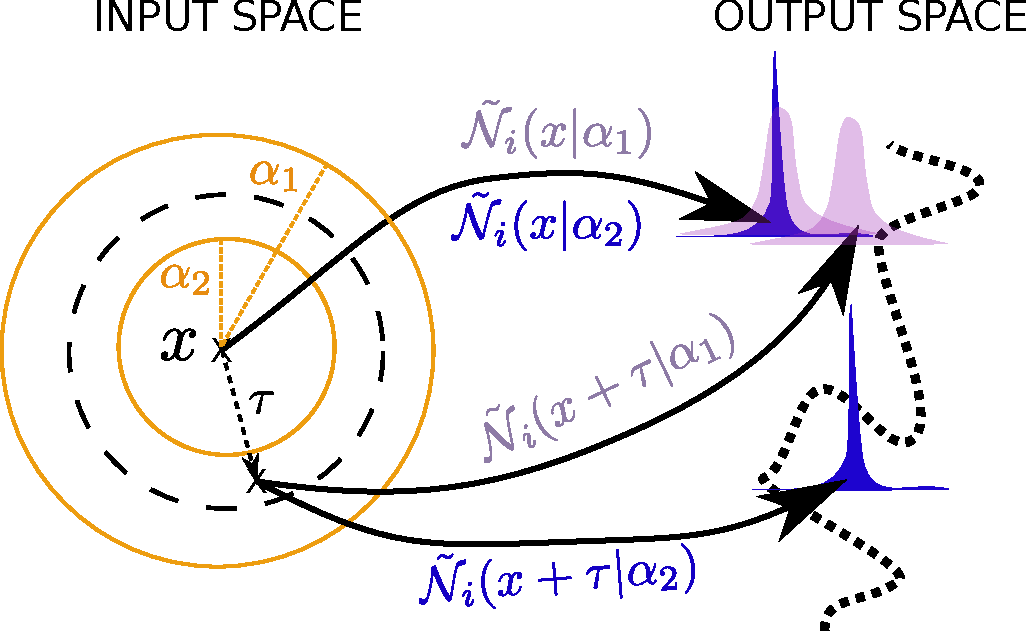
\includegraphics[width=0.5\columnwidth]{images/advAttackRobustV5.pdf}}
% \caption{Illustration of the robustness against adversarial examples for probabilistic mappings (that map images to ditributions).}
% \label{robustness_fig}
% \end{center}
% \vskip -0.2in
% \end{figure}

%$x$ is a natural image and $x+\tau$ an adversarial attack on $x$.  The input space is the space of natural images $\mathcal{X}$, and the output space is the image of $\mathcal{X}$ by the $i$-th layer of the network $\Tilde{\mathcal{N}}_i$. The dashed circle in the input space represents the maximal amount of noise keeping the adversarial example visually close from $x$, and the dashed line in the output space represents the embedding of the decision boundary in the output space of $\mathcal{N}_i$.




% \subsection{On the need for injecting noise in the training phase}
% \label{section::covariateshift}

% So far, we have  designed an algorithm for neural networks to ensure robustness at inference time. But simply injecting noise at inference time destroys the accuracy of the algorithm. Thus one needs to also inject noise during the training phase as well. The justification comes from the distribution shift~\citep{sugiyama2012machine}.
% Distribution shift occurs when the training distribution differs from the test distribution. This implies that the hypothesis minimizing the empirical risk is not consistent, i.e. it does not converge to the true model as the training size increases. A way to circumvent that is to ensure that training and test distributions matches using importance weighting (in the case of covariate-shift) or with noise injection in training and test phases (in our case).
%Let $f$ be the target function one wants to learn, The goal of supervised learning is to approximate this function by a parametrized function $\hat{f}_{\theta}$ from a training dataset $\{(x_i^{tr},y_i^{tr})\}_{i=1}^{n_{tr}}$ i.i.d sampled from an underlying distribution $p_{tr}$. When considering a problem of supervised learning, one assume that the training distribution $p_{tr}$ is actually the same distribution the test distribution $p_{te}$. However, this assumption is not always fulfilled. Situations where training and test datasets follow different distributions are called covariate shift. The interested reader should refer to~\citep{sugiyama2012machine} for a complete introduction on machine learning under covariate shift.
% \Jam{Remove the sequel and put it in the appendice
% The standard method to learn the parameter $\theta$ is the empirical risk minimization (ERM):
% $$\hat{\theta}_{ERM} := \text{argmin}_{\theta}\left[\frac{1}{n_{tr}} \sum_{ i =1}^{n_{tr}} \ell \left(y_i^{tr},\hat{f}_{\theta}\left(x_i^{tr}\right)\right)\right]$$

% where $\ell$ is the loss function at hand.
% The model is said to be correctly specified if there exists a parameter $\theta^{*}$ such that $\hat{f}_{\theta^{*}}=f$. Otherwise, the model is said to be misspecified. It is usually hard to design correctly specified models in machine learning. Hence it is useful to separate models into consistent and non consistent models. 
% A correctly specified model is said to be consistent if $\hat{\theta}_{ERM}$ converges in probability to $\theta^{*}$, as $n_{tr} \rightarrow \infty$. A misspecified model is said to be consistent if it converges to the parameter minimizing the generalization error $$G(\theta) := \mathbb{E}_{(x^{te},y^{te})\sim p_{te}}\left[\ell\left(y^{te},\hat{f}_{\theta}\left(x^{te}\right)\right)\right].$$

% %Since $G(\theta)$ is usually hard to obtain, to evaluate the performance of the obtained model, one can process the empirical generalization error using a test dataset $\{(x_i^{te},y_i^{te})\}_{i=1}^{n_{te}}$ i.i.d sampled from $p_{te}$. 
% %$ G(\theta) = \mathbb{E}_{(X,Y)\sim p_{te}}\left[\ell\left(Y,\hat{f}_{\theta}\left(X\right)\right)\right] $

% If $p_{tr}=p_{te}$, $\hat{\theta}_{ERM}$ is proven to be consistent, but it is not under distribution shift (i.e when $p_{tr}\neq p_{te}$). In fact, ERM remains consistent when the model is correctly specified, but no longer if the model is misspecified . For the sake of readability, for the remaining of this work we denote $\hat{f}:=\hat{f}_{\hat{\theta}_{ERM}}$. 
% }

%\subsection{Bound on the accuracy drop of the method}
\subsubsection{Bound on the risk gap under attack and certified accuracy}

The notions of risk and adversarial risk can easily be generalized to encompass probabilistic mappings. % (e.g by analogy with PAC Bayes theory).

\begin{definition}[Risks for probabilistic mappings]
 Let $\probmap$ be a probabilistic mapping from $\mathcal{X}$ to $\mathcal{Y}$, the risk and the $\varepsilon$-radius adversarial risk of $\probmap$ w.r.t. $\mathcal{D}$ are defined as:
 \begin{align*}
&\risk(\probmap):= \mathbb{E}_{(x,y)\sim \mathcal{D}}\left[ \mathbb{E}_{y'\sim \probmap(x)} \left[ \mathds{1} \left( y' \neq y \right)\right]\right]\\
&\riskadv(\probmap):= \mathbb{E}_{(x,y)\sim \mathcal{D}}\left[ \sup_{\lVert{\tau}\rVert_{\mathcal{X}} \leq \varepsilon}\mathbb{E}_{y'\sim \probmap(x+\tau)} \left[ \mathds{1} \left( y' \neq y \right)\right]\right]\enspace.
\end{align*}
% Regarding the randomization of neural networks, we define the following notions of generalization. For $\Tilde{\mathcal{N}}^i_X$ a randomized neural network with some noise $X$ injected at layer $i$ in:
% \begin{itemize}


%     % \item  Generalization error: $Err(\mathcal{N})=\mathbb{E}_{(x,y)}(1\!\!1_{\mathcal{N}(x)\neq y})$

%     % \item Adversarial generalization error: $Err_\varepsilon(\mathcal{N})=\mathbb{E}_{(x,y)}(\sup_{\tau/\norm{\tau}\leq\varepsilon}1\!\!1_{\mathcal{N}(x+\tau)\neq y})$

%     \item Generalization error for the probabilistic mapping $\Tilde{\mathcal{N}}^i_X$: 
    
%     $$\overline{Err}(\Tilde{\mathcal{N}}^i_X)=\mathbb{E}_{(x,y)}(\mathbb{E}_{X}(1\!\!1_{\Tilde{\mathcal{N}}^i_X(x)\neq y}))$$%=\mathbb{E}_{X}(Err(\Tilde{\mathcal{N}}^i_X))$$
    
%     \item Adversarial generalization error for the probabilistic mapping $\Tilde{\mathcal{N}}^i_X$:
    
%     $$\overline{Err}_\varepsilon(\Tilde{\mathcal{N}}^i_X)=\mathbb{E}_{(x,y)}(\sup_{\tau/\norm{\tau}\leq\varepsilon}\mathbb{E}_{X}(1\!\!1_{\Tilde{\mathcal{N}}^i_X(x+\tau)\neq y}))$$%=\mathbb{E}_{X}(Err_\varepsilon(\Tilde{\mathcal{N}}^i_X))$$
% \end{itemize}

\end{definition}


The definition of adversarial risk for a probabilistic mapping can be matched with the concept of Expectation over Transformation (EoT) attacks~\citep{athalye2018obfuscated}. Indeed, EoT attacks aim at computing the best opponent in expectation for a given random transformation. In the adversarial risk definition, the adversary chooses the perturbation which has the greatest probability to fool the model, which is a stronger objective than the EoT objective. Theorem~\ref{thm:bound} provides a bound on the gap between the adversarial risk and the regular risk:

\begin{thm}[Adversarial risk gap bound in the randomized setting]

\label{thm:bound}
Let $\probmap$ be the probabilistic mapping at hand. Let us suppose that  $\probmap$ is $d_{R,\lambda}$-$(\varepsilon,\alpha)$ robust for some $\lambda\geq1$ then:

$$|\riskadv(\probmap)-\risk(\probmap)|\leq 1-e^{-\alpha}\mathbb{E}_x\left[e^{-H(\probmap(x))}\right]$$
where $H$ is the Shannon entropy $H(p)=-\sum_i p_i \log(p_i)\enspace.$
\end{thm}
This theorem gives a control on the loss of accuracy under attack w.r.t. the robustness parameter $\alpha$ and the entropy of the predictor. It provides a tradeoff between the quantity of noise added in the network and the accuracy under attack. Intuitively, when the noise increases, for any input, the output distribution tends towards the uniform distribution, then, $\alpha\rightarrow0$ and $H(\probmap(x))\rightarrow \log(K)$, and the risk and the adversarial risk both tends to $\frac{1}{K}$ where $K$ is the number of classes in the classification problem. On the opposite, if no noise is injected, for any input, the output distribution is a  Dirac distribution, then, if the prediction for the adversarial example is not the same as for the regular one, $\alpha\rightarrow\infty$ and $H(\probmap(x))\rightarrow 0$. Hence, the noise needs to be designed both to preserve accuracy and robustness to adversarial attacks. In the Section~\ref{section::experiment}, we give an illustration of this bound when $\probmap$ is a neural network with noise injection at input level as presented in Theorem~\ref{thm:netrob}. In practice, we do not have access to the real value of the  entropy, but we estimate it with classical estimators~\citep{paninski2003estimation}.

Our framework being general enough it encompasses several known accuracy certificates from the literature, e.g. the one provided in~\citep{lecuyer2018certified}. Interestingly, we can introduce the following one, based on \emph{our} definition of robustness. 

\begin{thm}
\label{thm::Lecuyerlike}
Let $x \in \mathcal{X}$, and $\probmap$ be a probabilistic mapping with values in $\mathbb{R}^{K}$. If $\probmap$ is $d_{R,\lambda}$-$(\varepsilon,\alpha)$ robust, and if there exist $k^{*}$ and $ \delta^{*} \in (0,1)$ s.t. $\mathbb{E}_{y \sim \probmap(x)}\left[ y_{k^{*}} \right] > e^{2\alpha'} \max\limits_{i \neq k^{*}}\mathbb{E}_{y \sim \probmap(x)}\left[ y_i \right] + (1+ e^{\alpha'})\delta^{*}$, with $\alpha'= \alpha + \frac{\log(1/\delta^{*})}{\lambda - 1}$. Then, for the classifier $ f: x \mapsto \argmaxB\limits_{k \in [K]}\mathbb{E}_{y \sim \probmap(x)}\left[ y_k \right]$ there is no perturbation $\tau \in B(0,\varepsilon)$ such that $f(x)\neq f(x+\tau)$. 
\end{thm}

As the main focus of this work is to give theoretical evidence for randomization techniques, numerical experiments will mainly focus on Theorem~\ref{thm:netrob} and~\ref{thm:bound} and not on certificates (Theorem~\ref{thm::Lecuyerlike}). %illustrating the results from Theorem~\ref{thm:netrob} and Theorem~\ref{thm:bound}.


% \begin{align*}
% |\overline{Err}_\varepsilon(\mathcal{\Tilde{N}}_X^i)-\overline{Err}(\mathcal{\Tilde{N}}_X^i)|  &= |\mathbb{E}_{(x,y)}( \sup_{\tau/\norm{\tau}\leq\varepsilon} \mathbb{E}_X(1\!\!1_{\Tilde{\mathcal{N}}^i_X(x+\tau)\neq y})-  \mathbb{E}_X(1\!\!1_{\Tilde{\mathcal{N}}^i_X(x)\neq y}))| \\
% &=|\mathbb{E}_{(x,y)}( \sup_{\tau/\norm{\tau}\leq\varepsilon} \mathbb{E}_{X_1,X_2}(1\!\!1_{\Tilde{\mathcal{N}}^i_{X_1}(x+\tau)\neq y}-  1\!\!1_{\Tilde{\mathcal{N}}^i_{X_2}(x)\neq y}))|\\
% &\leq\mathbb{E}_{(x,y)}( \sup_{\tau/\norm{\tau}\leq\varepsilon} \mathbb{E}_{X_1,X_2}(|1\!\!1_{\Tilde{\mathcal{N}}^i_X(x+\tau)\neq y}-  1\!\!1_{\Tilde{\mathcal{N}}^i_X(x)\neq y}|))\\
% &=\mathbb{E}_{(x,y)}(\sup_{\tau/\norm{\tau}\leq\varepsilon}\mathbb{P}_{X_1,X_2}(\Tilde{\mathcal{N}}^i_{X_1}(x+\tau)=\Tilde{\mathcal{N}}^i_{X_2}(x)))
% \end{align*}



% where $X_1$ and $X_2$ are two independent samples with the same law than $X$.

% For two discrete random independent variables of law $P=(p_1,...,p_K)$ and $Q=(q_1,...,q_K)$: 
% $$\mathbb{P}(P=Q)=\sum_{i=1}^K p_i q_i \geq \exp{(\sum_{i=1}^K p_i \log q_i)}=\exp{(-d_{KL}(P||Q)-H(P))}$$



\subsection{Numerical experiments}
\label{section::experiment}
To illustrate our theoretical findings, we train randomized neural networks with a simple method which consists in injecting a noise drawn from an Exponential family distribution in the image during training and inference. 
\subsubsection{Experimental setup}
We present our results and analysis on  CIFAR-10, CIFAR-100 \citep{krizhevsky2009learning} and ImageNet datasets \citep{imagenet_cvpr09}. For CIFAR-10 and CIFAR-100 \citep{krizhevsky2009learning}, we used a Wide ResNet architecture \citep{ZagoruykoK16} which is a variant of the ResNet model from \citep{He_2016_CVPR}. We use 28 layers with a widen factor of 10. We train all networks for 200 epochs, a batch size of 400, dropout 0.3 and Leaky Relu activation with a slope on $\mathbb{R}^-$ of 0.1. We minimize the Cross Entropy Loss with Momentum 0.9 and use a piecewise constant learning rate of 0.1, 0.02, 0.004 and 0.00008 after respectively 7500, 15000 and 20000 steps. The networks achieve for CIFAR10 and 100 a TOP-1 accuracy of 95.8\% and 79.1\% respectively on test images. For ImageNet \citep{imagenet_cvpr09}, we use an Inception ResNet v2 \citep{szegedy2017inception} which is the sate of the art architecture for this dataset and achieve a TOP-1 accuracy of 80\%. For the training of ImageNet, we use the same hyper parameters setting as the original implementation. We train the network for 120 epochs with a batch size of 256, dropout 0.8 and Relu as activation function. All evaluations were done with a single crop on the non-blacklisted subset of the validation set.

To transform these classical networks to probabilistic mappings, we inject noise drawn from Laplace and Gaussian distributions, each with various standard deviations. While the noise could theoretically be injected anywhere in the network, we inject the noise on the image for simplicity. More experiments with noise injected in the first layer of the network are presented in the supplementary material. To evaluate our models under attack, we use three powerful iterative attacks with different norms: \emph{ElasticNet} attack (EAD)~\citep{chen2018ead} with $\ell_1$ distortion, \emph{Carlini\&Wagner} attack (C\&W)~\citep{carlini2017towards} with $\ell_2$ distortion and \emph{Projected Gradient Descent} attack (PGD)~\citep{madry2017towards} with $\ell_\infty$ distortion. All standard deviations and attack intensities are in between $-1$ and $1$. Precise descriptions of our numerical experiments and of the attacks used for evaluation are deferred to the supplementary material. 

\textbf{Attacks against randomized defenses:} It has been pointed out by \citep{athalye2017synthesizing,carlini2019evaluating} that in a white box setting, an attacker with a complete knowledge of the system will know the distribution of the noise injected in the network. As such, to create a stronger adversarial example, the attacker can take the expectation of the loss or the logits of the randomized network during the computation of the attack. This technique is called Expectation Over Transformation ($\EoT$) and we use a Monte Carlo method with $80$ simulations to approximate the best perturbation for a randomized network. 

\subsubsection{Experimental results}



\begin{figure}[t]
\centering
\subfigure[]{
    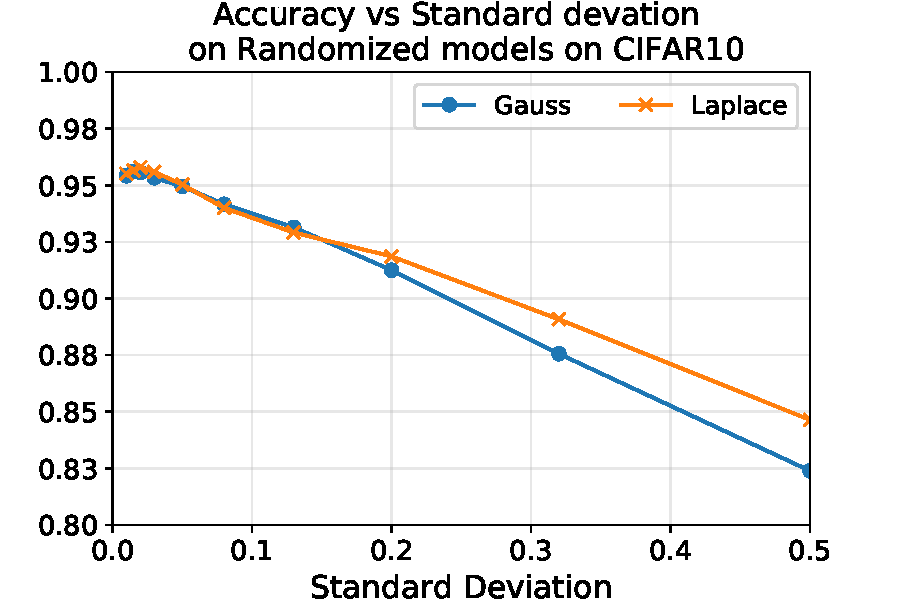
\includegraphics[width=.31\textwidth]{sections/4_certification/images/acc_sd_CIFAR10.pdf}
    \label{fig:acc_sd_CIFAR10}
    }
\subfigure[]{
    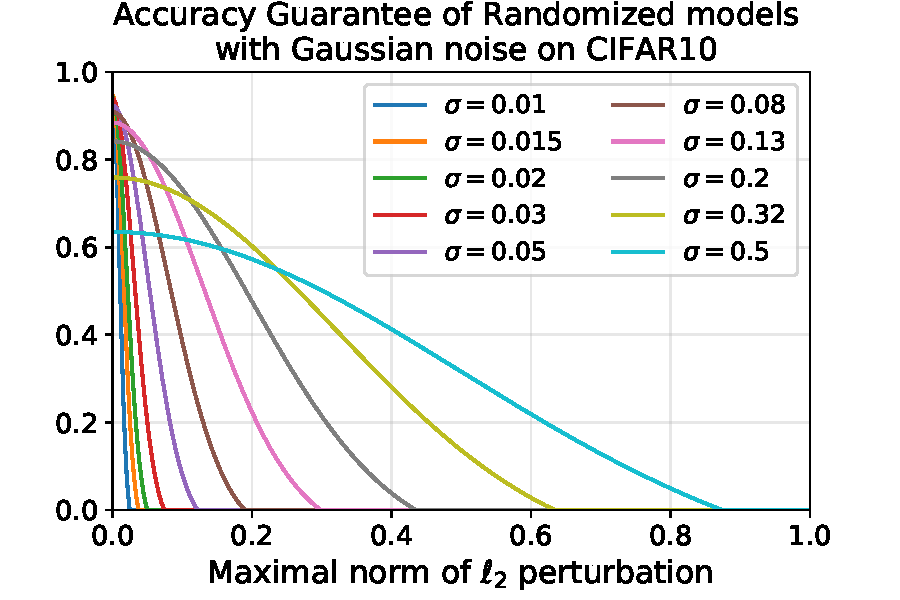
\includegraphics[width=.31\textwidth]{sections/4_certification/images/gauss_certif_CIFAR10.pdf}
    \label{fig:gauss_certif_CIFAR10}
    }
\subfigure[]{
    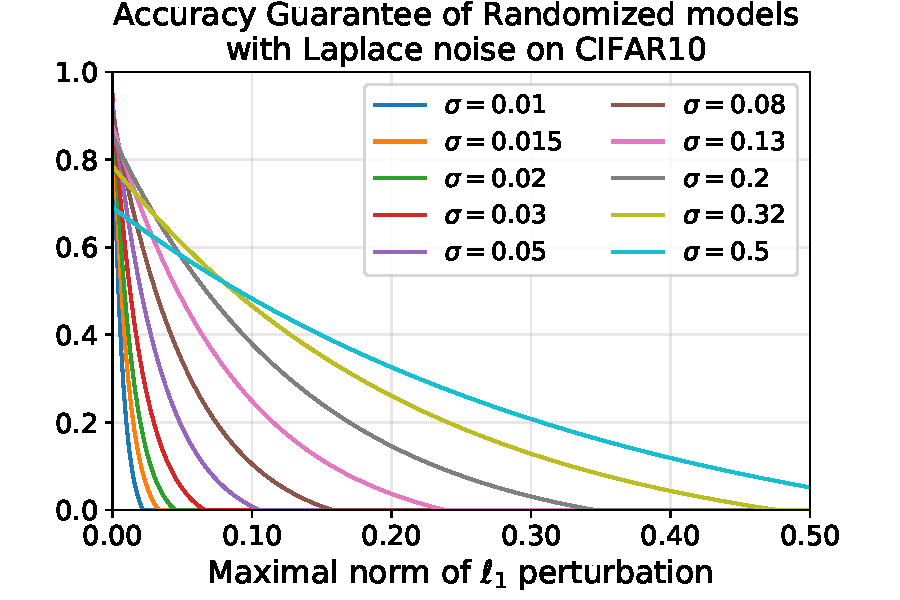
\includegraphics[width=.31\textwidth]{sections/4_certification/images/laplace_certif_CIFAR10.pdf}
    \label{fig:laplace_certif_CIFAR10}
    }
\caption{(a) Impact of the standard deviation of the injected noise on accuracy in a randomized model on CIFAR-10 with a Wide ResNet architecture. (b) and (c) illustration of the guaranteed accuracy of different randomized models with Gaussian (b) and Laplace (c) noises given the norm of the adversarial perturbation. The accuracies and entropies and estimated empirically. \label{fig:cifar10_results}
}
\end{figure}
\textbf{Trade-off between accuracy and intensity of noise:} When injecting noise as a defense mechanism, regardless of the distribution it is drawn from, we observe (as in Figure~\ref{fig:acc_sd_CIFAR10}) that the accuracy decreases when the noise intensity grows. In that sense, noise needs to be calibrated to preserve both accuracy and robustness against adversarial attacks, i.e. it needs to be large enough to preserve robustness and small enough to preserve accuracy. Figure~\ref{fig:acc_sd_CIFAR10} shows the loss of accuracy on CIFAR10 from $0.95$ to $0.82$ (respectively $0.95$ to $0.84$) with noise drawn from a Gaussian distribution (respectively Laplace) with a standard deviation from $0.01$ to $0.5$. Figure~\ref{fig:gauss_certif_CIFAR10} and \ref{fig:laplace_certif_CIFAR10} illustrate the theoretical lower bound on accuracy under attack of Theorem~\ref{thm:bound} for different distributions and standard deviations. The term in entropy of Theorem~\ref{thm:bound} has been estimated using a Monte Carlo method with $10^4$ simulations. The trade-off between accuracy and robustness from Theorem~\ref{thm:bound} thus appears w.r.t the noise intensity. With small noises, the accuracy is high, but the guaranteed accuracy drops fast w.r.t the magnitude of the adversarial perturbation. Conversely, with bigger noises, the accuracy is lower but decreases slowly w.r.t the magnitude of the adversarial perturbation. These Figures also show that Theorem~\ref{thm:bound} gives strong accuracy guarantees against small adversarial perturbations. Next paragraph shows that in practice, randomized networks achieve much higher accuracy under attack than the theoretical bound, and against much larger perturbations.

\textbf{Performance of randomized networks under attacks and comparison to state of the art:}\label{sec:perf_under_attack} While Figure~\ref{fig:gauss_certif_CIFAR10} and \ref{fig:laplace_certif_CIFAR10} illustrated a theoretical robustness against growing adversarial perturbations, Table~\ref{tab:accuracy_under_attack} illustrates this trade-off experimentally. It compares the accuracy under attack of a deterministic network with the one of randomized networks with Gaussian and Laplace noises both with low ($0.01$) and high ($0.5$) standard deviations. Randomized networks with a small noise lead to no loss in accuracy with a small robustness while high noises lead to a higher robustness at the expense of loss of accuracy ($\sim11$ points). Table~\ref{table:madry_vs_random} compares the accuracy and the accuracy under attack of randomized networks with Gaussian and Laplace distributions for different standard deviations against adversarial training~\citep{madry2017towards}. We observe that the accuracy on natural images of both noise injection methods are similar to the one from~\citep{madry2017towards}. Moreover, both methods are more robust than adversarial training to PGD and C\&W attacks. With all the experiments, to construct an $\EoT$ attack,  we use 80 Monte Carlo simulations at every step the attacks. These experiments show that randomized defenses can be competitive given the intensity of noise injected in the network. Note that these experiments have been led with $\EoT$ of size 80. For much bigger sizes of $\EoT$ these results would be mitigated. Nevertheless, the accuracy would never drop under the bounds illustrated in Figure~\ref{fig:cifar10_results}, since Theorem~\ref{thm:bound} gives a bound that on the worst case attack strategy (including $\EoT$).  

\begin{table}[t]
  \centering
  \caption{Accuracy under attack on the CIFAR-10 dataset with a randomized Wide ResNet architecture. We compare the accuracy on natural images and under attack with different noise over 3 iterative attacks (the number of steps is next to the name) made with 80 Monte Carlo simulations to compute EoT attacks. The first line is the baseline, no noise has been injected.}
    \begin{tabular}{lccccc}
    \toprule
    \textbf{Distribution} & \textbf{Sd} & \textbf{Natural} & \textbf{$\ell_1$ -- EAD 60} & \textbf{$\ell_2$ -- C\&W 60} & \textbf{$\ell_\infty$ -- PGD 20} \\
    \midrule
    - & - & 0.958 & 0.035 & 0.034 & 0.384 \\
    \midrule
    \multirow{2}[0]{*}{Normal} & 0.01 & 0.954 & 0.193 & 0.294 & 0.408 \\
          & 0.50 & 0.824 & 0.448 & 0.523 & 0.587 \\
    \midrule
    \multirow{2}[0]{*}{Laplace} & 0.01 & 0.955 & 0.208 & 0.313 & 0.389 \\
          & 0.50 & 0.846 & 0.464 & 0.494 & 0.589 \\
    \bottomrule
    \end{tabular}%
  \label{tab:accuracy_under_attack}%
\end{table}%



% \subsection{Comparison with Adversarial Training (Q4)}\label{sec:adv_madry}

\begin{table}[t]
  \caption{Accuracy under attack of randomized neural network with different distributions and standard deviations versus adversarial training by Madry et al. \citep{madry2017towards}. The PGD attack has been made with 20 step, an epsilon of 0.06 and a step size of 0.006 (input space between $-1$ and $+1$). The Carlini\&Wagner attack uses 30 steps, 9 binary search steps and a 0.01 learning rate. The first line refers to the baseline without attack.}
  \label{Results}
  \centering
  \begin{tabular}{ccccccc}
    \toprule
      & & \multirow{2}[0]{*}{\citep{madry2017towards}} & \multirow{2}[0]{*}{\textbf{Normal 0.32}} & \multirow{2}[0]{*}{\textbf{Laplace 0.32}} & \multirow{2}[0]{*}{\textbf{Normal 0.5}} & \multirow{2}[0]{*}{\textbf{Laplace 0.5}} \\
     \textbf{Attack} & \textbf{Steps} & & & \\
    \midrule
    -  & - & 0.873 & 0.876 & 0.891 & 0.824 & 0.846 \\ 
    $\ell_\infty$ -- PGD & 20 & 0.456 & 0.566 & 0.576 & 0.587 & 0.589 \\
    $\ell_2$ -- C\&W & 30 & 0.468 & 0.512 & 0.502 & 0.489 & 0.479 \\
    \bottomrule
  \end{tabular}
  \label{table:madry_vs_random}
\end{table}


% \subsection{Conclusion and future work}
% \label{section::conclusion}
% This paper brings new contributions to the field of provable defenses to adversarial attacks. Principled answers have been provided to key questions on the interest of randomization techniques, and on their loss of accuracy under attack. The obtained bounds have been illustrated in practice by conducting thorough experiments on baseline datasets such as CIFAR and ImageNet. We show in particular that a simple method based on injecting noise drawn from the Exponential family is competitive compared to baseline approaches while leading to provable guarantees. Future work will focus on investigating other noise distributions belonging or not to the Exponential family, combining randomization with more sophisticated defenses and on devising new tight bounds on the adversarial risk gap.

% \textbf{Acknowledgements: }  This work was granted access to the OpenPOWER prototype from GENCI-IDRIS under the Preparatory Access AP010610510 made by GENCI. R. Pinot benefited from a JSPS Summer Program Fellowship during this work (Grant number SP18218). L. Meunier and J. Atif would also like to thank Adrien Balp from Société Générale for his support.

%Our work contributes to the body of work on defense strategies through randomization by answering key questions on the interest of the Exponential family as a noise generating family and on the adversarial generalization gap bound for associated randomized networks. The bounds are only effective on low dimensional images/limited size perturbations because the ratio between an adversarial perturbation norm and the standard deviation of the injected noise increases as the dimension grows. However, the experimental results are encouraging on every datasets (including ImageNet). Future work will focus on investigating other noise families, combining randomization with more involved defenses and on devising new tight bounds on the adversarial generalization gap. 

% %Injecting noise drawn from an Exponential family in a neural network  has proved its efficiency both from theoretical and experimental standpoints. 
% Our work contributes to the body of work on defense strategies through randomization by answering key questions on the interest of the Exponential family as a noise generating family and on the adversarial generalization gap bound for associated randomized networks.  
% %randomized networks~\citep{lecuyer2018certified,KolterRandomizedSmoothing} that propose a certificate, by presenting a guarantee on the drop of accuracy under attacks for $\ell_2$  or $\ell_1$ norms. It also provides principled arguments supporting the use of randomization as a defense technique.  
% But so far, as for former works, the provided guarantees only hold for small size perturbations. Moreover, the theoretical bounds are only effective on low dimensional images as CIFAR because the ratio between an adversarial perturbation norm and the noise standard deviation of the injected noise rapidly increases as the dimension grows. However, the experimental results are encouraging on every dataset including ImageNet. %It has also been shown that these methods also present a trade-off between accuracy and adversarial robustness. 
% Future work will focus on investigating other noise families, belonging to or beyond the Exponential family, combining the randomization technique with more involved defenses (e.g. adversarial training, ensembles, etc.) and on devising new tight bounds on the adversarial gap. 

%Most empirical defenses against adversarial attacks have been defeated~\citep{athalye2018obfuscated}. Compared to these methods, randomized networks have the advantage to provide theoretical guarantees and to be independent from the neural architecture of the networks. Randomized techniques also experimentally scale well to higher dimension inputs and seem to provide equivalent or better results than classical adversarial training. In future work, we plan to investigate more complex architectures, other noise injection schemes and even the combination with other defenses~\citep{madry2018towards,goodfellow2014explaining}. But more importantly, we aim at developing new family of noise (respecting conditions of Theorem~\ref{thm:netrob}) further impeding the loss of accuracy.

%This is a cool paper

% % donner un cadre theotrique pour comprendre pourquoi les methodes prec d'injection de bruit
% In this work, we bring a theoretically well-grounded framework in order to understand why previous methods based on noise injection were in practice effective against adversarial attacks.  While the very article is a theoretical analysis, it also paves the way to novel defense mechanisms using noises from yet unexplored distributions.
% %In this work, we propose a theoretical insight on why randomizing neural networks makes them more robust against adversarial attacks. We provide a simple methodology that ensures the classifier to be robust. We have proved the wide class of Exponential family distributions can be used to defend against adversarial attacks.

% Our theoretical analysis mainly focused on the robustness of the methods but our numerical experiments validated that the accuracy was slightly altered by noise injection. Hence, we demonstrated the practical applicability of the approach. Note also that as we only used a vanilla ResNet21, using tricks of the trade for neural networks and the noise injection, the accuracy could be further improved.
% %We provided experiments to support our results and we clearly improve robustness by injecting noise at a layer in a feed forward neural network. However, there still exists a trade off between the noise intensity and the accuracy: adding noise increases robustness against adversarial attacks but weakens the accuracy of the classifier. But so far, even a small intensity noise helps defending against adversarial attacks without loosing a lot of accuracy. 

% In future work, we plan to investigate more complex architectures, other noise injection schemes and even the combination with other defenses~\citep{madry2018towards,goodfellow2014explaining}. But more importantly, we aim at developing new family of noise (respecting conditions of Theorem~\ref{thm:netrob}) further impeding the loss of accuracy.


\newpage


\section{Introduction}

Modern neural networks have been known to be sensible against small, imperceptible and adversarially-chosen perturbations of their inputs~\citep{biggio2013evasion,szegedy2014intriguing}.
This vulnerability  has become a major issue as more and more neural networks have been deployed into production applications.
Over the past decade, the research progress plays out like a cat-and-mouse game between the development of more and more powerful attacks~\citep{goodfellow2014explaining,kurakin2016adversarial,carlini2017adversarial,croce2020reliable} and the design of empirical defense mechanisms~\citep{madry2017towards,moosavi2019robustness,cohen2019certified}.
Finishing the game calls for certified adversarial robustness~\citep{raghunathan2018certified,wong2018scaling}.
While recent work devised defenses with theoretical guarantees against adversarial perturbations, they share the same limitation, \ie, the tradeoffs between expressivity and robustness, and between scalability and accuracy.

A natural approach to provide robustness guarantees on a classifier is to enforce Lipschitzness properties. 
To achieve such properties, researchers mainly focused on two different kinds of approaches.
The first one is based on randomization~\citep{lecuyer2018certified,cohen2019certified,pinot2019theoretical} and consists in convolving the input with with a predefined probability distribution.
While this approach offers some level of scalability (\ie, currently the only certified defense on the ImageNet dataset), it suffers from significant impossibility results~\cite{yang2020randomized}.
A second approach consists in building $1$-Lipschitz layers using specific linear transform~\citep{cisse2017parseval,li2019preventing,anil2019sorting,trockman2021orthogonalizing,skew2021sahil,li2019preventing,singla2021householder}.
Knowing the Lipschitz constant of the network, it is then possible to compute a certification radius around any points. 

A large line of work explored the interpretation of residual neural networks \cite{he2016deep} as a parameter estimation problem of nonlinear dynamical systems~\citep{haber2017stable,e17Proposal,lu18beyond}.
Reconsidering the ResNet architecture as an Euler discretization of a continuous dynamical system yields to the trend around Neural Ordinary Differential Equation~\citep{chen2018neural}.
For instance, in the seminal work of~\citet{haber2017stable}, the continuous formulation offers more flexibility to investigate the stability of neural networks during inference, knowing that the discretization will be then implemented by the architecture design.
The notion of stability, in our context, quantifies how a small perturbation on the initial value impacts the trajectories of the dynamical system. 

From this continuous and dynamical interpretation, we  analyze the Lipschitzness property of Neural Networks. We then study the discretization schemes that can preserve the Lipschitzness properties. With this point of view, we can readily recover several previous methods that build 1-Lipschitz neural networks~\citep{trockman2021orthogonalizing,skew2021sahil}.
Therefore, the dynamical system perspective offers a general and flexible framework to build Lipschitz Neural Networks facilitating the discovery of new approaches.
In this vein, we introduce convex potentials in the design of the Residual Network flow and show that this choice of parametrization yields to by-design $1$-Lipschitz neural networks.
At the very core of our approach lies a new $1$-Lipschitz non-linear operator that we call {\em Convex Potential Layer} which allows us to adapt convex potential flows to the discretized case. 
These blocks enjoy the desirable property of stabilizing the training of the neural network by controlling the gradient norm, hence overcoming the exploding gradient issue.
We experimentally demonstrate our approach by training large-scale neural networks on several datasets, reaching state-of-the art results in terms of under-attack and certified accuracy.



\section{Background and Related Work}
\label{section:background_rw}

In this paper, we aim at devising {\em certified} defense mechanisms against adversarial attacks, in the following, we formally define an adversarial attacks and a robustness certificate.
We consider a classification task from an input space $\mathcal{X}\subset\RR^d$ to a label space $\mathcal{Y}:=\{1,\dots,K\}$.
To this end, we aim at learning a classifier function $\mathbf{f}:=(f_1,\dots,f_K):\mathcal{X}\to \RR^K$ such that the predicted label for an input $x$ is $\argmaxB_k f_k(x)$.
For a given couple input-label $(x,y)$, we say that $x$ is correctly classified if $\argmaxB_k f_k(x)=y$.


\begin{definition}[{\bf Adversarial Attacks}]
Let $x \in \mathcal{X}$, $y \in \mathcal{Y}$ the label of $x$ and let $\mathbf{f}$ be a classifier.
An adversarial attack at level $\varepsilon$ is a perturbation $\tau$ \st $\lVert\tau\rVert\leq\varepsilon$ such that:
\begin{equation*}
  \argmaxB_k f_k(x+\tau) \neq y
\end{equation*}
\end{definition}
Let us now define the notion of  robust certification. For $x \in \mathcal{X}$, $y \in \mathcal{Y}$ the label of $x$ and let $\mathbf{f}$ be a classifier, a classifier $\mathbf{f}$ is said to be \emph{certifiably robust at radius $\varepsilon\geq 0$} at point $x$ if for all $\tau$ such that ${\lVert\tau\rVert \leq \varepsilon}$ :
\begin{equation*}
  \argmaxB_k f_k(x+\tau) = y
\end{equation*}
The task of robust certification is then to find methods that ensure the previous property. A key quantity in this case is the Lipschitz constant of the classifier.



\subsection{Lipschitz property of Neural Networks}

The Lipschitz constant has seen a growing interest in the last few years in the field of deep learning~\citep{scaman2018lipschitz,fazlyab2019efficient,combettes2020lipschitz,bethune2021many}.
Indeed, numerous results have shown that neural networks with a small Lipschitz constant exhibit better generalization~\citep{bartlett2017spectrally}, higher robustness to adversarial attacks~\citep{szegedy2014intriguing,farnia2018generalizable,tsuzuku2018lipschitz}, better training stability~\citep{xiao2018dynamical,trockman2021orthogonalizing}, improved Generative Adversarial Networks~\citep{arjovsky2017wasserstein}, etc.
Formally, we define the Lipschitz constant with respect to the $\ell_2$ norm of a Lipschitz continuous function $f$ as follows:
\begin{equation*}
  Lip_{2}{(f)} = \sup_{\substack{x, x' \in \mathcal{X} \\ x \neq x'}} \frac{\lVert f(x) - f(x') \rVert_2}{\lVert x - x' \rVert_2} \enspace.
\end{equation*}

Intuitively, if a classifier is Lipschitz, one can bound the impact of a given input variation on the output, hence obtaining guarantees on the adversarial robustness.
We can formally characterize the robustness of a neural network with respect to its Lipschitz constant with the following proposition:
\begin{prop}[\citet{tsuzuku2018lipschitz}] \label{proposition:tsuzuku}
Let $\mathbf{f}$ be an $L$-Lipschitz continuous classifier for the $\ell_2$ norm.
Let $\varepsilon > 0$, $x \in \mathcal{X}$ and $y \in \mathcal{Y}$ the label of $x$.
If at point $x$, the margin $\mathcal{M}_{\mathbf{f}}(x)$ satisfies:
\begin{equation*}
  \mathcal{M}_{\mathbf{f}}(x):=\max(0,f_y(x)-\max_{y'\neq y}f_{y'}(x)) > \sqrt{2} L \varepsilon
\end{equation*}
then we have for every $\tau$ such that $\lVert \tau \rVert_2 \leq \varepsilon$:
\begin{equation*}
  \argmaxB_{k}f_k(x + \tau) = y
\end{equation*}
\end{prop}
From Proposition~\ref{proposition:tsuzuku}, it is straightforward to compute a robustness certificate for a given point.
Consequently, in order to build robust neural networks the margin needs to be large and the Lipschitz constant small to get optimal guarantees on the robustness for neural networks.



\subsection{Certified Adversarial Robustness}

Mainly two kinds of methods have been developed to come up with certified adversarial robustness.
The first category relies on randomization and consists of convolving the input with a predefined probability distribution during both training and inference phases.
Several works that rely on the method have proposed empirical~\cite{cao2017mitigating,liu2018towards,pinot2019theoretical,pinot2020randomization} and certified defenses~\cite{lecuyer2018certified,li2019certified,cohen2019certified,salman2019provably,yang2020randomized}. These methods are model-agnostic, in the sense they do not depend on the architecture of the classifier, and provide ``high probability'' certificates.
However, this approach suffers from significant impossibility results: the maximum radius that can be certified for a given smoothing distribution vanishes as the dimension increases~\cite{yang2020randomized}.
Furthermore, in order to get non-vacuous provable guarantees, such approaches often require to query the network hundreds of times to infer the label of a single image.
This computational cost naturally limits the use of these methods in practice.

The second approach directly exploits the Lipschitzness property with the design of built-in $1$-Lipschitz layers. Contrarily to previous methods,  these approaches provide deterministic guarantees.
Following this line, one can either normalize the weight matrices by their largest singular values making the layer $1$-Lipschitz, \emph{e.g.}~\citep{yoshida2017spectral,miyato2018spectral,farnia2018generalizable,anil2019sorting} or project the weight matrices on the Stiefel manifold \citep{li2019preventing,trockman2021orthogonalizing,skew2021sahil}.
The work of \citet{li2019preventing}, \citet{trockman2021orthogonalizing} and \citet{skew2021sahil} (denoted BCOP, Cayley and SOC respectively) are considered the most relevant approach to our work.
Indeed, their approaches consist of projecting the weights matrices onto an orthogonal space in order to preserve gradient norms and enhance adversarial robustness by guaranteeing low Lipschitz constants. 
While both works have similar objectives, their execution is different.
The BCOP layer (Block Convolution Orthogonal Parameterization) uses an iterative algorithm proposed by \citet{bjorck1971iterative} to orthogonalize the linear transform performed by a convolution.
The SOC layer (Skew Orthogonal Convolutions) uses the property that if $A$ is a skew symmetric matrix then $Q=\exp{A}$ is an orthogonal matrix. To approximate the exponential, the authors proposed to use a finite number of terms in its Taylor series expansion.
Finally, the method proposed by~\citet{trockman2021orthogonalizing} use the Cayley transform to orthogonalize the weights matrices.
Given a skew symmetric matrix $A$, the Cayley transform consists in computing the orthogonal matrix $Q = (I - A)^{-1} (I + A)$. Both methods are well adapted to convolutional layers and are able to reach high accuracy levels on CIFAR datasets. Also, several works~\cite{anil2019sorting,singla2021householder,huang2021local} proposed methods leveraging the properties of activation functions to constraints the Lipschitz of Neural Networks. These works are usually useful to help  improving the performance of linear orthogonal layers.


\subsection{Residual Networks}

To prevent from gradient vanishing issues in neural networks during the training phase~\citep{hochreiter2001gradient},~\cite{he2016deep} proposed the Residual Network (ResNet) architecture.
Based on this architecture, several works~\citep{haber2017stable,e17Proposal,lu18beyond,chen2018neural} proposed a ``continuous time'' interpretation inspired by dynamical systems that can be defined as follows.

\begin{definition}\label{def:flow}
Let $(F_{t})_{t\in[0,T]}$ be a family of functions on $\RR^d$, we define the continuous time Residual Networks flow associated with $F_t$ as:
\begin{align*}\label{eq:resnet_c0}
  \left\{
    \begin{array}{ll}
    x_0 &= x\in\mathcal{X}\\
    \frac{dx_{t}}{dt} &= F_{{t}}(x_{t}) \  \text{for } \ t\in[0, T]
  \end{array}
  \right.
\end{align*}
\end{definition}

This continuous time interpretation helps as it allows us to consider the stability of the forward propagation through the stability of the associated dynamical system.
A dynamical system is said to be \emph{stable} if two trajectories starting from an input and another one remain sufficiently close to each other all along the propagation.
This stability property takes all its sense in the context of adversarial classification.

It was argued by~\citet{haber2017stable} that when $F_{t}$ does not depend on $t$ or vary slowly with time\footnote{This blurry definition of "vary slowly" makes the property difficult to apply.}, the stability can be characterized by the eigenvalues of the Jacobian matrix $\nabla_x F_{t}(x_t)$: 
the dynamical system is stable if the real part of the eigenvalues of the Jacobian stay negative throughout the propagation.
This property however only relies on intuition and this condition might be difficult to  verify in practice.
In the following, in order to derive stability properties, we study gradient flows and convex potentials, which are sub-classes of Residual networks.

Other works~\citep{huang2020adversarial,li2020implicit} also proposed to enhance adversarial robustness using dynamical systems interpretations of Residual Networks. Both works argues that using particular discretization scheme would make gradient attacks more difficult to compute due to numerical stability. These works did not provide any provable guarantees for such approaches.



\section{A Framework to design Lipschitz Layers}
\label{section:global_framework}


The continuous time interpretation of Definition~\ref{def:flow} allows us to better investigate the robustness properties and assess how a difference of the initial values (the inputs) impacts the inference flow of the model. Let us consider two continuous flows $x_t$ and $z_t$ associated with $F_t$ but differing in their respective initial values $x_0$ and $z_0$. Our goal is to characterize the time evolution of $\lVert x_t-z_t \rVert$ by studying its  time derivative. We recall that  every matrix $M\in\RR^{d\times d}$ can be uniquely decomposed as the sum of a symmetric and skew-symmetric matrix $M = S(M) + A(M)$. By applying this decomposition to the Jacobian matrix $\nabla_x F_t(x)$ of $F_t$, we can show that the time derivative of $\lVert x_t-z_t \rVert$ only involves the symmetric part  $S(\nabla_x F_t(x))$ (see Appendix~\ref{proof:continuous-lip} for details). 

For two symmetric matrices $S_1,S_2\in\RR^{d\times d}$,  we denote $S_1\preceq S_2$ if, for all $x\in\RR^d$, $\langle x,(S_2-S_1)x\rangle\geq 0$. By focusing on the symmetric part of the Jacobian matrix we can show in Appendix~\ref{proof:continuous-lip} the following proposition.
\begin{prop}
\label{prop:continuous-lip}
Let $(F_{t})_{t\in[0,T]}$ be a family of differentiable  functions almost everywhere on $\RR^d$.
Let us assume that there exists two measurable functions $t\mapsto \mu_t$ and  $t\mapsto \lambda_t$ such that
$$\mu_t I\preceq S(\nabla_xF_{t}(x))\preceq \lambda_tI$$
for all $x\in\RR^d$, and $t\in [ 0,T]$. Then the flow associated with $F_t$ satisfies for all initial conditions $x_0$ and $z_0$:
\begin{align*}
  \lVert x_0-z_0 \rVert e^{\int_0^t\mu_s ds}\leq \lVert x_t-z_t \rVert\leq \lVert x_0-z_0 \rVert e^{\int_0^t\lambda_s ds}
\end{align*}
\end{prop}

The symmetric part plays even a more important role since one can show that a function whose Jacobian is always skew-symmetric is actually linear (see Appendix~\ref{sup:skew} for more details). However, constraining $S(\nabla_x F_{t}(x))$ in the general case is technically difficult and a solution resorts to a more intuitive parametrization of  $F_t$ as the sum of two functions $F_{1,t}$ and $F_{2,t}$ whose Jacobian matrix are respectively symmetric  and skew-symmetric.  Thus, such a parametrization enforces $F_{2,t}$  to be linear and skew-symmetric. For the choice of $F_{1,t}$, we propose to rely on potential functions: a function  $F_{1,t}:\RR^d \to \RR^d$ derives from a simpler family of scalar valued function in $\RR^d$, called the \emph{potential}, via the gradient operation. Moreover, since the Hessian of the potential is symmetric, the Jacobian for $F_{1,t}$ is then also symmetric.  If we had the convex property to this potential, its Hessian has positive eigenvalues. Therefore we introduce the following corollary. See proof in Appendix~\ref{proof:conv-skew} 

\begin{corollary} 
\label{cor:conv-skew}Let $(f_{t})_{t\in[0,T]}$ be a family of convex differentiable functions on $\RR^d$ and $(A_t)_{t\in[0,T]}$ a family of skew symmetric matrices. Let us define 
$$F_t(x) = -\nabla_x f_{t}(x)+A_t x,$$ 
then the flow associated with $F_t$ satisfies for all initial conditions $x_0$ and $z_0$:
\begin{align*}
\lVert x_t-z_t \rVert\leq \lVert x_0-z_0 \rVert
\end{align*}
\end{corollary}

This simple property suggests that if we could parameterize $F_t$  with convex potentials, it would be less sensitive to input perturbations and therefore more robust to adversarial examples. We also remark that the skew symmetric part is then norm-preserving.
However, the discretization of such flow is challenging in order to maintain this property of stability. 


\subsection{Discretized Flows}

To study the discretization of  the previous flow, let $t=1,\dots,T$ be the discretized time steps and from now we consider the flow defined by  $F_t(x) = -\nabla f_{t}(x)+A_t x$, with $(f_{t})_{t=1,\dots,T}$  a family of convex differentiable functions on $\RR^d$ and $(A_t)_{t=1,\dots,T}$ a family of skew symmetric matrices. The most basic method the explicit Euler scheme as defined by: 
\begin{align*}
x_{t+1} = x_t+ F_t(x_t)
\end{align*}
However, if $A_t\neq 0$, this discretized system might not satisfy $\lVert x_t-z_t\rVert\leq\lVert x_0-z_0\rVert$. Indeed, consider the simple example where $f_t=0$. We then have:
\begin{align*}
\lVert x_{t+1}-z_{t+1}\rVert - \lVert x_{t}-z_{t}\rVert =\lVert A_t\left(x_{t}-z_{t}\right)\rVert.
\end{align*}
Thus explicit Euler scheme cannot guarantee Lipschitzness when $A_t\neq 0$. To overcome this difficulty, the discretization step can be split in two parts, one for $\nabla_x f_t$ and one for $A_t$: 
\begin{align*}
   \left\{
    \begin{array}{ll}
        x_{t+\frac12} &= \textsc{step1}(x_t, \nabla_x f_t)\\
        x_{t+1}& = \textsc{step2}(x_{t+\frac12}, A_t)
    \end{array} 
    \right.
\end{align*}
This type of discretization scheme  can be found for instance from Proximal Gradient methods where one step is explicit and the other is implicit. Then, we dissociate the Lipschitzness study of both terms of the flow. 

\subsection{Discretization scheme for $\nabla_x f_t$}

To apply the explicit Euler scheme to $\nabla_x f_t$, an  additional smoothness property on the potential functions is required  to generalize the Lipschitzness guarantee to the discretized flows. Recall that a function $f$ is said to be \emph{$L$-smooth} if it is differentiable and if $x\mapsto\nabla_x f(x)$ is $L$-Lipschitz. 
\begin{prop}\label{prop:discrete_convex_potentials}
Let $t\in\{1,\cdots,T\}$ Let us assume that $f_{t}$ is $L_t$-smooth. We  define the following discretized ResNet gradient flow using $h_t$ as a step size:
\begin{align*}
    \begin{array}{ll}
    x_{t+\frac12} &= x_{t}-h_{t}\nabla_xf_{t}(x_{t})\\
  \end{array}
 \end{align*}
Consider now two trajectories $x_t$ and $z_t$ with initial points $x_0=x$ and $z_0=z$ respectively,  if $0\leq h_t\leq \frac{2}{L_t}$,  then 
$$\lVert x_{t+\frac12}-z_{t+\frac12}\rVert_2\leq \lVert x_t-z_t\rVert_2$$
\end{prop}
In Section~\ref{sec:param}, we describe how to parametrize a neural network layer to implement such a discretization step by leveraging the recent work on Input Convex Neural Networks~\cite{amos2017input}. 

\begin{rmq}
Another solution relies on the implicit Euler scheme: $ x_{t+\frac12} = x_{t}-\nabla_xf_{t}(x_{t+\frac12})$. We show in Appendix~\ref{sup:implicit} that this strategy defines a $1$-Lipschitz flow without further assumption on $f_t$ than convexity. We propose an implementation. However preliminary experiments did not show competitive results and the training time is prohibitive. We leave this solution for future work. 

\end{rmq}
\subsection{Discretization scheme for $A_t$}

The second step of discretization involves the term with skew-symmetric matrix $A_t$. As mentioned earlier, the challenge is that the \emph{explicit Euler discretization} is not contractive. More precisely,  the following property 
$$\lVert x_{t+1} - z_{t+1}\rVert\geq \lVert x_{t+\frac12} - z_{t+\frac12}\rVert$$ 
is satisfied with equality only in the special and useless case of $x_{t+\frac12} - z_{t+\frac12} \in \text{ker}(A_t)$. Moreover, the implicit Euler discretization induces an increasing norm and hence does not satisfy the desired property of norm preservation neither. 

\paragraph{Midpoint Euler method.}
We thus propose to use \emph{Midpoint Euler} method, defined as follows:
\begin{align*}
&x_{t+1} = x_{t+\frac12} +A_t \frac{x_{t+1}+x_{t+\frac12}}{2}\\
\iff&x_{t+1} = \left(I-\frac{A_t}{2}\right)^{-1}\left(I+\frac{A_t}{2}\right)x_{t+\frac12}.
\end{align*} 
Since $A_t$ is skew-symmetric, $I-\frac{A_t}{2}$ is invertible. This update corresponds to the Cayley Transform of $\frac{A_t}{2}$ that induces an orthogonal mapping. 
This kind of layers was introduced and extensively studied in~\citet{trockman2021orthogonalizing}.  


\paragraph{Exact Flow.} One can define the simple differential equation corresponding to the flow associated with $A_t$  
\begin{align*}
        \frac{du_t}{ds} = A_t u_s,\quad u_0 = x_{t+\frac12},
\end{align*}
There exists an exact solution exists since $A_t$ is linear. By taking the value at $s=\frac12$, we obtained the following transformation:  
 \begin{align*}
x_{t+1} := u_{\frac12}=e^{\frac{A}{2}} x_{t+\frac12}.
\end{align*}
This step is therefore clearly norm preserving but the matrix exponentiation is challenging and it requires efficient approximations. This trend was recently investigated under the name of Skew Orthogonal Convolution (SOC)~\cite{skew2021sahil}.


\section{Parametrizing Convex Potentials Layers}
\label{sec:param}

As presented in the previous section, parametrizing the skew symmetric updates has been extensively studied by~\citet{trockman2021orthogonalizing,skew2021sahil}. In this paper we focus on  the parametrization of symmetric update with the convex potentials proposed in~\ref{prop:discrete_convex_potentials}. For that purpose, the Input Convex Neural Network (ICNN) \citep{amos2017input} provide a relevant starting point that we will extend. 

\subsection{Gradient of ICNN}
We use $1$-layer ICNN~\citep{amos2017input} to define an efficient computation of Convex Potentials Flows. For any vectors $w_1,\dots w_k\in\mathbb{R}^d$, and bias terms  $b_1,\dots,b_k\in \mathbb{R}$, and for $\phi$ a convex function,  the potential $F$ defined as:
\begin{align*}
    F_{w,b}:x\in\RR^d\mapsto \sum_{i=1}^k\phi( w_i^\top x+b_i)
\end{align*}
defines  a convex function in $x$ as the composition of a linear and a convex function. Its gradient with respect to its input $x$ is then:
\begin{align*}
    x\mapsto \sum_{i=1}^kw_i\phi'(w_i^\top x+b_i) = \mathbf{W}^\top \phi'(\mathbf{W} x+\mathbf{b})
\end{align*}
with $\mathbf{W}\in \mathbb{R}^{k\times d}$ and $\mathbf{b}\in\mathbb{R}^{k}$ are respectively the matrix and vector obtained by the concatenation of, respectively, $w_i^\top$ and $b_i$, and $\phi'$ is applied element-wise.  
Moreover, assuming $\phi'$ is $L$-Lipschitz, we have that $F_{w,b}$ is  $L\lVert\mathbf{W}\rVert_2^2$-smooth. $\lVert\mathbf{W}\rVert_2$ denotes the spectral norm of $\mathbf{W}$.
% , \ie, the greatest singular value of $\mathbf{W}$ defined as:
% \begin{align*}
%    \lVert\mathbf{W}\rVert_2 :=\max_{x\neq 0} \frac{\lVert \mathbf{W}x\rVert_2}{\lVert x\rVert_2}
% \end{align*}
The reciprocal also holds: if $\sigma:\RR\to\RR$ is a non-decreasing $L$-Lipschitz function, $\mathbf{W}\in \RR^{k\times d}$ and $b\in \RR^{k}$, there exists a convex $L\lVert\mathbf{W}\rVert_2^2$-smooth function $F_{w,b}$ such that 
$$\nabla_xF_{w,b}(x) =  \mathbf{W}^\top \sigma(\mathbf{W} x+\mathbf{b}),$$ where $\sigma$ is applied element-wise. The next section shows how this property can be used to implement the building block and training of such layers. 


\subsection{Convex Potential layers}
From the previous section, we derive the following \emph{Convex Potential Layer}: 
\begin{equation*}
\label{equation:stable_block}
  z = x - \frac{2}{\lVert \mathbf{W} \lVert_2^2} \mathbf{W}^\top \sigma(\mathbf{W} x + b)
\end{equation*}
Written in a matrix form, this layer can be implemented with every linear operation $\mathbf{W}$.
In the context of image classification, it is beneficial to use convolutions\footnote{For instance, one can leverage the \texttt{Conv2D} and \texttt{Conv2D\_transpose} functions of the PyTorch framework~\citep{paszke2019pytorch}} instead of generic linear transforms represented by a dense matrix. 

\begin{rmq}
When $\mathbf{W}\in\RR^{1\times d}$, $b =0$ and $\sigma=\textsc{ReLU}$, the \emph{Convex Potential Layer} is equivalent to the HouseHolder activation function introduced in~\citet{singla2021householder}.
\end{rmq}

Residual Networks~\citep{he2016deep} are also composed of other types of layers which increase or decrease the dimensionality of the flow.
Typically, in a classical setting, the number of input channels is gradually increased, while the size of the image is reduced with pooling layers.
In order to build a $1$-Lipschitz Residual Network, all operations need to be properly scale or normalize in order to maintain the Lipschitz constant.

\paragraph{Increasing dimensionsionality.} To increase the number of channels in a convolutional Convex Potential Layer, a zero-padding operation can be easily performed: an input $x$ of size $c\times h \times w$ can be extended to some $x'$ of size  $c'\times h \times w$, where $c'>c$, which equals $x$ on the $c$ first channels and $0$ on the $c'-c$ other channels.
\paragraph{Reducing dimensionsionality.} Dimensionality reduction is another essential operation in neural networks. On one hand, its  goal is to  reduce the number of parameters and thus the amount of computation required to build the network. On the other hand it allows the model to progressively map the input space on the output dimension, which corresponds in many cases to the number of different labels $K$. 
In this context, several operations exist:
pooling layers are used to extract information present in a region of the feature map generated by a convolution layer. One can easily adapt pooling layers (\emph{e.g.} max and average) to make them $1$-Lipschitz~\citep{bartlett2017spectrally}.
Finally, a simple method to reduce the dimension is the product with a non-square matrix. In this paper, we simply implement it as  the truncation of the output. This obviously maintains the Lipschitz constant.


\begin{algorithm}[tb]
\caption{Computation of a Convex Potential Layer}
\label{algorithm:stable_block}
\begin{algorithmic}
  \STATE{Require: \bfseries Input: $x$, vector: $u$, weights: $\mathbf{W}$, $b$}
  \STATE{Ensure: Compute the layer $z$ and return $u$}
  \STATE{$v \gets \mathbf{W} u / \lVert \mathbf{W} u \rVert_2$}
  \STATE{$u \gets \mathbf{W}^\top v / \lVert \mathbf{W}^\top v \rVert_2$
    \rlap{\hspace{0.5cm}\smash{$\left.\begin{array}{@{}c@{}}\\{}\\{}\end{array}\right\}%
      \begin{tabular}{l}1 iter. for training \\100 iter. for inference\end{tabular}$}}}
  \STATE{$h \gets 2 / \left( \sum_i (\mathbf{W} u \cdot v)_i \right)^2$}
  \STATE{\textbf{return} $x - h \left[ \mathbf{W}^\top \sigma( \mathbf{W} x + b) \right], u$}
\end{algorithmic}
\end{algorithm}




\subsection{Computing spectral norms}
Our Convex Potential Layer, described in Equation~\ref{equation:stable_block}, can be adapted to any kind of linear transformations (\emph{i.e.} Dense or Convolutional) but requires the computation of the spectral norm for these transformations.
Given that computation of the spectral norm of a linear operator is known to be NP-hard~\citep{steinberg2005computation}, an efficient approximate method is required during training to keep the complexity tractable. 


Many techniques exist to approximate the spectral norm (or the largest singular value), and most of them exhibit a trade-off between efficiency and accuracy.
Several methods exploit the structure of convolutional layers to build an upper bound on the spectral norm of the linear transform performed by the convolution~\citep{jia2017improving,singla2021fantastic,araujo2021lipschitz}.
While these methods are generally efficient, they can less relevant and adapted to certain settings. For instance in our context, using a loose upper bound of the spectral norm will hinder the expressive power of the layer and make it too contracting.

For these reasons we rely on the Power Iteration Method (PM).  This method converges at a geometric rate towards the largest singular value of a matrix. More precisely the convergence rate for a given matrix $\mathbf{W}$ is $\textstyle O((\frac{\lambda_2}{\lambda_1})^k)$ after $k$ iterations, independently from the choice for the starting vector, where $\lambda_1>\lambda_2$ are the two largest singular values of $\mathbf{W}$. While it can appear to be computationally expensive due to the large number of required iterations for convergence, it is possible to drastically reduce the number of iterations during training. Indeed, as in~\citep{miyato2018spectral}, by considering that the weights' matrices $\mathbf{W}$ change slowly during training, one can perform only one iteration of the PM for each step of the training and let the algorithm slowly converges along with the training process\footnote{Note that a typical training requires approximately 200K steps where 100 steps of PM is usually enough for convergence}.
We describe with more details in Algorithm~\ref{algorithm:stable_block}, the operations performed during a forward pass with a Convex Potential Layer. 

However for evaluation purpose, we need to compute the certified adversarial robustness, and this requires to ensure the convergence of the PM. Therefore, we perform $100$ iterations for each layer\footnote{$100$ iterations of Power Method is sufficient to converge with a geometric rate.} at inference time. Also note that at inference time, the computation of the spectral norm only needs to be performed once for each layer. 



\section{Experiments}
\label{section:experiments}
\begin{table}
\begin{center}
    \begin{tabular}{cccccccc}
    \toprule
    \textbf{\#} & \textbf{S} &  & \textbf{M} & & \textbf{L} & & \textbf{XL} \\
    \midrule
    \textbf{Conv. Layers}      & 20 & & 30 & & 50& & 70 \\
    \textbf{Channels}  &45 & & 60 & & 90 & & 120 \\ 
    \textbf{Lin. Layers}        &7 & & 10 & & 15 & & 15 \\
    \textbf{Lin. Features} & 2048 & & 2048 & & 4096 & & 4096 \\
    \bottomrule
    \end{tabular}%

\end{center}
\caption{\label{table:model-desc}
Architectures description for our Convex Potential Layers (CPL) neural networks with different capacities. We vary the number of Convolutional Convex Potential Layers, the number of Linear Convex Potential Layers, the number of channels in the convolutional layers and the width of fully
connected layers. They will be reported respectively as CPL-S, CPL-M, CPL-L and CPL-XL.}
\end{table}

To evaluate our new $1$-Lipschitz Convex Potential Layers, we conducted an extensive set of experiments. In this section, we first describe  the details of our experimental setup. We then recall  the concurrent approaches that build $1$-Lipschitz Neural Networks and stress their limitations. Our experimental results are finally summarized in Section~\ref{sec:setting-xp}. By computing the certified and empirical adversarial  accuracy of our networks on CIFAR10 and CIFAR100 classification tasks~\citep{krizhevsky2009learning}, we show that our architecture is competitive with state-of-the-art methods (Sections~\ref{sec:results}). We also study the influence of some hyperparameters and demonstrate the stability and the scalability of our approach by training very deep neural networks up to 1000 layers without normalization tricks or gradient clipping.










\subsection{Training and Architectural Details}
\label{sec:setting-xp}

We demonstrate the effectiveness of our approach on a classification task with CIFAR10 and CIFAR100 datasets~\citep{krizhevsky2009learning}. We use a similar training configuration to the one proposed in~\citep{trockman2021orthogonalizing}.
We trained our networks with a batch size of $256$ over $200$ epochs.
We use standard data augmentation (i.e. random cropping and flipping), a learning rate of $0.001$ with Adam optimizer \citep{diederik2014adam} without weight decay and a piecewise triangular learning rate scheduler. We used a margin parameter in the loss set to $0.7$.

As other usual convolutional neural networks, we first stack few Convolutional CPLs and then stack some Linear CPLs for classification tasks. To validate the performance  and the scalability of our layers,  we  evaluate four different variations of different hyperparameters as described in Table~\ref{table:model-desc}, respectively named CPL-S, CPL-M, CPL-L and CPL-XL, ranked according to the number of parameters they have. In all our experiments, we made $3$ independent trainings to evaluate accurately the models. All reported results are the average of these $3$ runs.

\subsection{Concurrent Approaches} We compare our networks with SOC~\citep{skew2021sahil} and Cayley~\cite{trockman2021orthogonalizing} networks which are to our knowledge the best performing approaches for deterministic $1$-Lipschitz Neural Networks. Since our layers are fundamentally different from these ones, we cannot compare with the same architectures. We reproduced SOC results for with $10$ and $20$ layers, that we call respectively SOC-$10$ and SOC-$20$ in the same training setting, {i.e.} normalized inputs, cross entropy loss, SGD optimizer with learning rate $0.1$ and multi-step learning rate scheduler. For Cayley layers networks, we reproduced their best reported model, {i.e.} KWLarge with width factor of $3$. 

The work of~\citet{singla2021householder} propose three methods to improve certifiable accuracies from SOC layers: a new HouseHolder activation function (HH),  last layer normalization (LLN), and certificate regularization (CR). The code associated with this approach is not open-sourced yet, so we just reported the results from their paper in ours results (Tables~\ref{table:c10-comp} and~\ref{table:c100-comp}) under the name SOC+. We were being able to implement the LLN method in all models. This method largely improve the result of all methods on CIFAR100, so we used it for all networks we compared on CIFAR100 (ours and concurrent approaches).


\begin{table*}[tb]
  \centering
  \sisetup{%
    table-align-uncertainty=true,
    separate-uncertainty=true,
    detect-weight=true,
    detect-inline-weight=math
  }
  \begin{tabular}
  {
    l
    S[table-format=2.2]
    S[table-format=2.2]
    S[table-format=2.2]
    S[table-format=2.2]
    S[table-format=2.2]
  }
  \toprule
    & \multicolumn{1}{c}{\textbf{Standard Accuracy}} & \multicolumn{3}{c}{\textbf{Provable Accuracy ($\varepsilon $)}} &  \multicolumn{1}{c}{\textbf{Time per epoch (s)}} 
    \\
    \cmidrule{3-5}
    & \multicolumn{1}{c}{ } & \multicolumn{1}{c}{36/255} & \multicolumn{1}{c}{72/255} &  \multicolumn{1}{c}{108/255} & \multicolumn{1}{c}{\textbf{}} 
    \\
  \midrule
    \textbf{CPL-S} & 75.6  & 62.3  & 46.9  & 32.2  & 21.9 \\
  \textbf{CPL-M} & 76.8  & 63.3  & 47.5  & 32.5  & 40.0 \\
  \textbf{CPL-L} & 77.7  & 63.9 & 48.1 & 32.9  & 93.4 \\
  \textbf{CPL-XL} & 78.5  & 64.4  & 48.0  & 33.0 & 163 \\
  \midrule
  \textbf{Cayley (KW3)} & 74.6  & 61.4  & 46.4  & 32.1  & 30.8\\
    \midrule

  \textbf{SOC-10} & 77.6  & 62.0  & 45.0  & 29.5  & 33.4 \\
  \textbf{SOC-20} & 78.0  & 62.7 & 46.0  & 30.3  &52.2\\
  \midrule
    \textbf{SOC+-10} & 76.2 &62.6 & 47.7 & 34.2& N/A\\
  \textbf{SOC+-20} & 76.3&62.6& 48.7& 36.0& N/A \\

  \bottomrule
  \end{tabular}%
  \caption{Results on the CIFAR10 dataset on standard and  provably certifiable accuracies for different values of perturbations $\varepsilon$ on CPL (ours), SOC and Cayley models. The average time per epoch in seconds is also reported in the last column. None of these networks uses Last Layer Normalization.}
  \label{table:c10-comp}%
\end{table*}%

\begin{table*}[tb]
  \centering
  \sisetup{%
    table-align-uncertainty=true,
    separate-uncertainty=true,
    detect-weight=true,
    detect-inline-weight=math
  }
  \begin{tabular}
  {
    l
    S[table-format=2.2]
    S[table-format=2.2]
    S[table-format=2.2]
    S[table-format=2.2]
    S[table-format=2.2]
  }
  \toprule
    & \multicolumn{1}{c}{\textbf{Standard Accuracy}} & \multicolumn{3}{c}{\textbf{Provable Accuracy ($\varepsilon $)}} &  \multicolumn{1}{c}{\textbf{Time per epoch (s)}} 
    \\
    \cmidrule{3-5}
    & \multicolumn{1}{c}{ } & \multicolumn{1}{c}{36/255} & \multicolumn{1}{c}{72/255} &  \multicolumn{1}{c}{108/255} & \multicolumn{1}{c}{\textbf{}} 
    \\
  \midrule
    \textbf{CPL-S} & 44.0  & 29.9  & 19.1  & 11.0  & 22.4 \\
  \textbf{CPL-M} & 45.6  & 31.1  & 19.3  & 11.3 & 40.7 \\
  \textbf{CPL-L} & 46.7  & 31.8 & 20.1  & 11.7  & 93.8 \\
  \textbf{CPL-XL} & 47.8  & 33.4  & 20.9  &  12.6  & 164 \\
  \midrule
  \textbf{Cayley (KW3)} & 43.3  & 29.2  & 18.8 & 11.0  & 31.3 \\
    \midrule

  \textbf{SOC-10} & 48.2  & 34.3  &22.7 & 14.0  & 33.8 \\
  \textbf{SOC-20} & 48.3  & 34.4 & 22.7  & 14.2 & 52.7 \\
  \midrule
    \textbf{SOC+-10} & 47.1& 34.5& 23.5& 15.7& N/A \\
  \textbf{SOC+-20} & 47.8 & 34.8 & 23.7 & 15.8 &  N/A\\

  \bottomrule
  \end{tabular}%
  \caption{Results on the CIFAR100 dataset on standard and  provably certifiable accuracies for different values of perturbations $\varepsilon$ on CPL (ours), SOC and Cayley models. The average time per epoch in seconds is also reported in the last column. All the reported networks use Last Layer Normalization.}
  \label{table:c100-comp}%
\end{table*}%


\subsection{Results}
\label{sec:results}


In this section, we present our results on adversarial robustness.
We provide results on provable $\ell_2$ robustness as well as empirical robustness on CIFAR10 and CIFAR100 datasets for all our models and the concurrent ones

\begin{figure}[h]
    \centering
    \begin{tabular}{cc}
    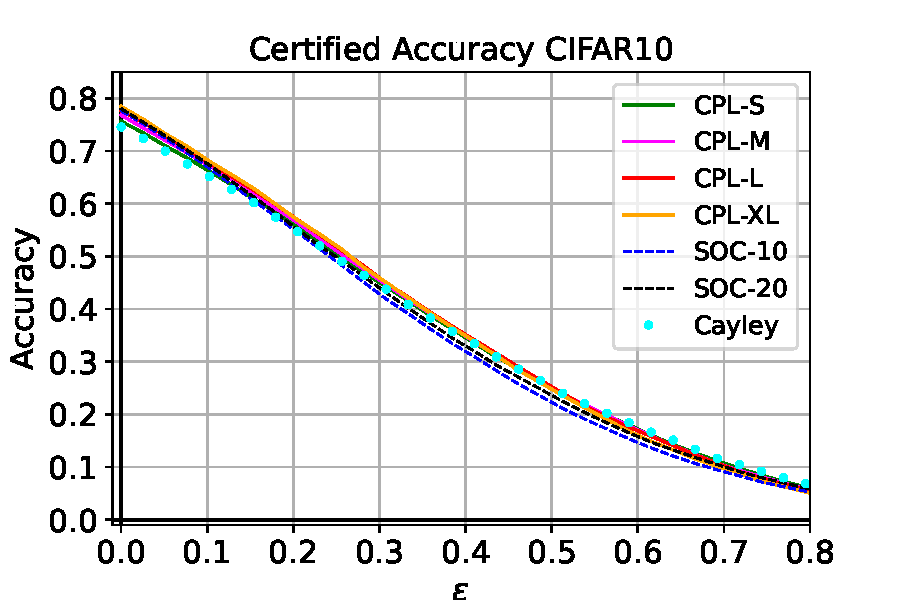
\includegraphics[width =0.48\textwidth]{sections/4_certification/images/cert_acc_eps_c10.pdf} & 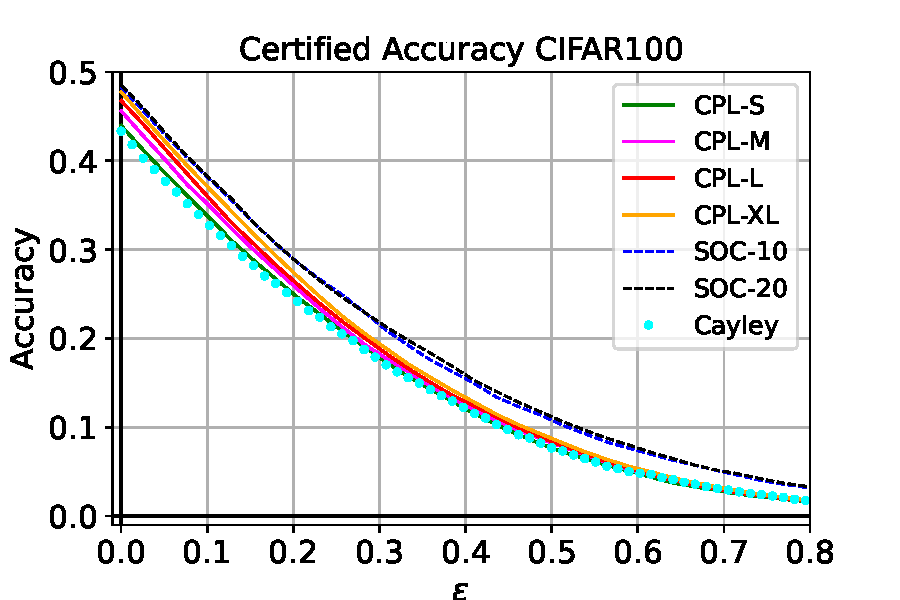
\includegraphics[width =0.48\textwidth]{sections/4_certification/images/cert_acc_eps_c100.pdf}
    \end{tabular}
    \caption{Certifiably robust accuracy  w.r.t. the perturbation $\varepsilon$ for our CPL networks and its concurrent approaches (SOC and Cayley models) on CIFAR10 and CIFAR100 datasets.}
    \label{fig:cert-acc}
\end{figure}

\paragraph{Certified Adversarial Robustness.} 
Results on CIFAR10 and CIFAR100 dataset are reported respectively in Tables~\ref{table:c10-comp} and~\ref{table:c100-comp}. We also plotted certified accuracy w.r.t. $\varepsilon$ on Figure~\ref{fig:cert-acc}. On CIFAR10, our method outperforms the concurrent approaches in terms of standard and certified accuracies for every level of $\varepsilon$ except SOC+ that uses additional tricks we did not use. On CIFAR100, our method performs slightly under the SOC networks but better than Cayley networks. Overall, our methods reach competitive results with SOC and Cayley layers. 

Note that we observe a small gain using larger and deeper architectures for our models. This gain is less important as $\varepsilon$ increases but the gain is non negligible for standard accuracies. In term of training time, our small architecture (CPL-S) trains very fast compared to other methods, while larger ones are longer to train.


\begin{figure}[h]
    \centering
    \begin{tabular}{cc}
    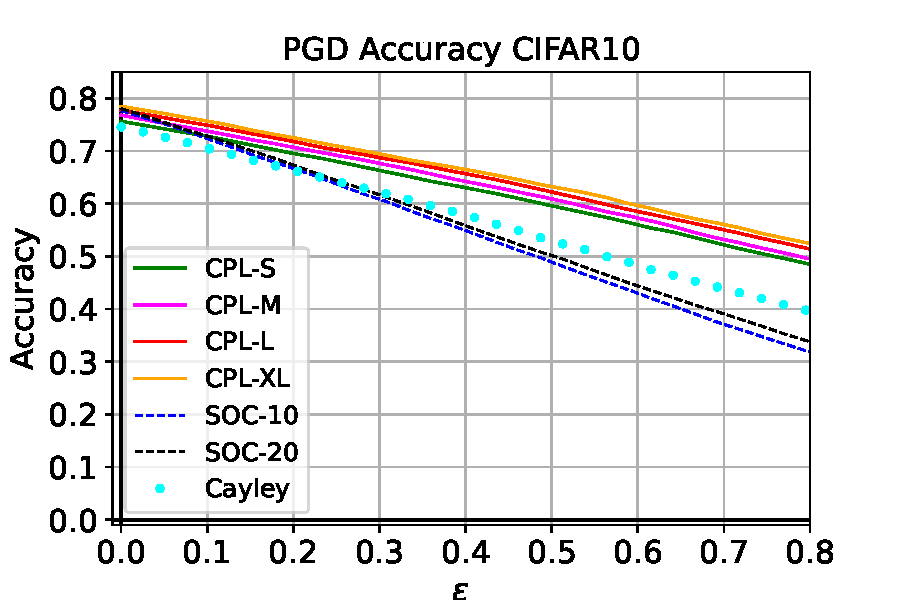
\includegraphics[width =0.48\textwidth]{sections/4_certification/images/pgd_acc_eps_c10.pdf} & 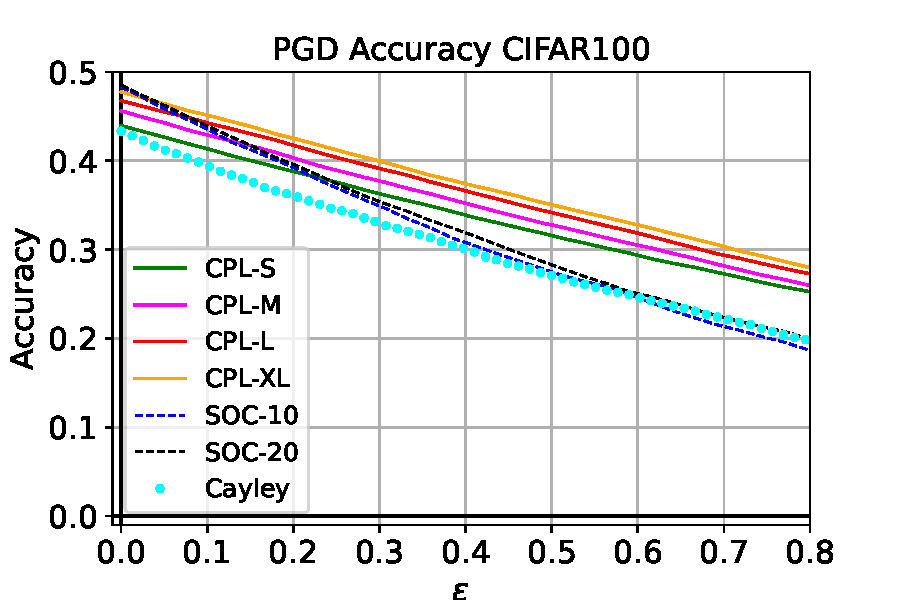
\includegraphics[width =0.48\textwidth]{sections/4_certification/images/pgd_acc_eps_c100.pdf}
    \end{tabular}
    \caption{Accuracy against PGD attack with 10 iterations w.r.t. the perturbation $\varepsilon$ for our CPL networks and its concurrent approaches on CIFAR10 and CIFAR100 datasets.}
    \label{fig:pgd-acc}
\end{figure}
\paragraph{Empirical Adversarial Robustness.} We also reported in Figure~\ref{fig:pgd-acc} the accuracy of all the models against PGD $\ell_2$-attack~\citep{kurakin2016adversarial,madry2018towards} for various levels of $\epsilon$. We used $10$ iterations for this attack. We remark here that our method brings a large gain of robust accuracy over all other methods. On CIFAR10 for $\varepsilon = 0.8$, the gain of CPL-S over SOC-10 approach is more than $10\%$. For CIFAR100, the gain is about $10\%$ too for $\varepsilon=0.6$. We remark that using larger architectures lead in a more substantial gain in empirical robustness. 

Our layers  only provide an upper bound on the Lipschitz constant, while orthonormal layers such as Cayley and SOC are built to exactly preserve the norms. This might negatively influence the certified accuracy since the effective Lipschitz constant is smaller than the theoretical one, hence leading to suboptimal certificates. This might explain why our method performs so well for empirical robustness tasks.






\begin{table*}[h]
  \centering
  \sisetup{%
    table-align-uncertainty=true,
    separate-uncertainty=true,
    detect-weight=true,
    detect-inline-weight=math
  }
  \begin{tabular}
  {
    l
    S[table-format=2.2]
    S[table-format=2.2]
    S[table-format=2.2]
    S[table-format=2.2]
    S[table-format=2.2]
    S[table-format=2.2]
  }
  \toprule
  &\multicolumn{1}{c}{\textbf{Batch}}& \multicolumn{1}{c}{\textbf{Standard Acc.}} & \multicolumn{3}{c}{\textbf{Provable Accuracy ($\varepsilon $)}} &  \multicolumn{1}{c}{\textbf{T./epoch (s)}} 
    \\
    \cmidrule{4-6}
    & \multicolumn{1}{c}{ } & \multicolumn{1}{c}{ } &\multicolumn{1}{c}{36/255} & \multicolumn{1}{c}{72/255} &  \multicolumn{1}{c}{108/255} & \multicolumn{1}{c}{\textbf{}} 
    \\
  \midrule
    \multirow{3}{*}{\textbf{CPL-S}} & 64 & 76.5& 62.9 & 47.3 & 32.0 & 48 \\
                                    & 128 & 76.1 & 62.8 & 47.1 & 32.3  & 31 \\
                                    & 256 & 75.6 & 62.3 & 46.9 & 32.2 & 22 \\
    \midrule
 \multirow{3}{*}{\textbf{CPL-M}} & 64 & 77.4 & 63.6 & 47.4 & 32.1  & 77 \\
                                    & 128 & 77.2 &63.5 & 47.5 & 32.1 & 50 \\
                                    & 256 & 76.8 & 63.2 & 47.4 & 32.4& 40 \\
    \midrule

 \multirow{3}{*}{\textbf{CPL-L}} & 64 & 78.4 & 64.2 & 47.8 & 32.2  & 162 \\
                                    & 128 & 78.2 & 64.3 & 47.9 & 32.5 & 109 \\
                                    & 256 & 77.6 & 63.9 & 48.1 & 32.7& 93 \\
  \midrule
 \multirow{3}{*}{\textbf{CPL-XL}} & 64 & 78.9 & 64.2 & 47.2 & 31.2  & 271 \\
                                    & 128 & 78.9 & 64.2 & 47.5 & 31.8 & 198 \\
                                    & 256 &78.5 & 64.4 & 47.8 & 32.4& 163 \\

  \bottomrule
  \end{tabular}%
  \caption{Results on the CIFAR10 dataset on standard and  provably certifiable accuracies for different values of perturbations $\varepsilon$ on CPL (ours) models with various batch sizes. The average time per epoch in seconds is also reported in the last column. All the reported networks use Last Layer Normalization.}
  \label{table:c10-comp-bs}%
\end{table*}%



\begin{table*}[h]
  \centering
  \sisetup{%
    table-align-uncertainty=true,
    separate-uncertainty=true,
    detect-weight=true,
    detect-inline-weight=math
  }
  \begin{tabular}
  {
    l
    S[table-format=2.2]
    S[table-format=2.2]
    S[table-format=2.2]
    S[table-format=2.2]
    S[table-format=2.2]
    S[table-format=2.2]
  }
  \toprule
  &\multicolumn{1}{c}{\textbf{Batch}}& \multicolumn{1}{c}{\textbf{Standard Acc.}} & \multicolumn{3}{c}{\textbf{Provable Acc. ($\varepsilon $)}} &  \multicolumn{1}{c}{\textbf{T./epoch (s)}} 
    \\
    \cmidrule{4-6}
    & \multicolumn{1}{c}{ } & \multicolumn{1}{c}{ } &\multicolumn{1}{c}{36/255} & \multicolumn{1}{c}{72/255} &  \multicolumn{1}{c}{108/255} & \multicolumn{1}{c}{\textbf{}} 
    \\
  \midrule
  \multirow{3}{*}{\textbf{CPL-S}} & 64 & 45,6 & 30,8 & 19,3 & 11,2 & 47 \\
                                    & 128 & 44,9 & 30,7 & 19,2 & 11,0 & 31\\
                                    & 256 & 44,0 & 29,9 & 19,1 & 10,9 & 23\\
  \midrule
  \multirow{3}{*}{\textbf{CPL-M}} & 64 & 46.6 & 31,6 & 19,6 & 11,6 & 78 \\
                                    & 128 & 46.3 & 31,1 & 19,7 & 11,5 & 55 \\
                                    & 256 & 45.6 & 31,1 & 19,3 & 11,3 & 41 \\

  \midrule

  \multirow{3}{*}{\textbf{CPL-L}} & 64 & 48.1 & 32,7 & 20,3 & 11,7 & 163 \\ 
                                    & 128 & 47,4 & 32,3 & 20,0 & 11,8 & 116 \\ 
                                    & 256 & 46,8 & 31,8 & 20,1 & 11,7 & 95 \\ 
  \midrule
  \multirow{3}{*}{\textbf{CPL-XL}} & 64 & 49,0 & 33,7 & 21,1 & 12,0 & 293 \\
                                    & 128 & 48,0 & 33,7 & 21,0 & 12,1 & 209 \\
                                    & 256 &47,8 & 33,4 & 20,9 & 12,6 & 164 \\

  \bottomrule
  \end{tabular}%
  \caption{Results on the CIFAR100 dataset on standard and  provably certifiable accuracies for different values of perturbations $\varepsilon$ on CPL (ours) models with various batch sizes. The average time per epoch in seconds is also reported in the last column. All the reported networks use Last Layer Normalization.}
  \label{table:c100-comp-bs}%
\end{table*}%

\paragraph{Effect of Batch Size in Training.}
In Tables~\ref{table:c10-comp-bs} and~\ref{table:c100-comp-bs}, we tried three different batch sizes (64, 128 and 256) for training our networks on CIFAR10 and CIFAR100 datasets, we remark a gain in standard accuracy in reducing the batch size for all settings. As the perturbation becomes larger, the gain in accuracy is reduced and even in some cases we may loose some points in robustness.





\begin{figure}[h]
    \centering
    \begin{tabular}{cc}
    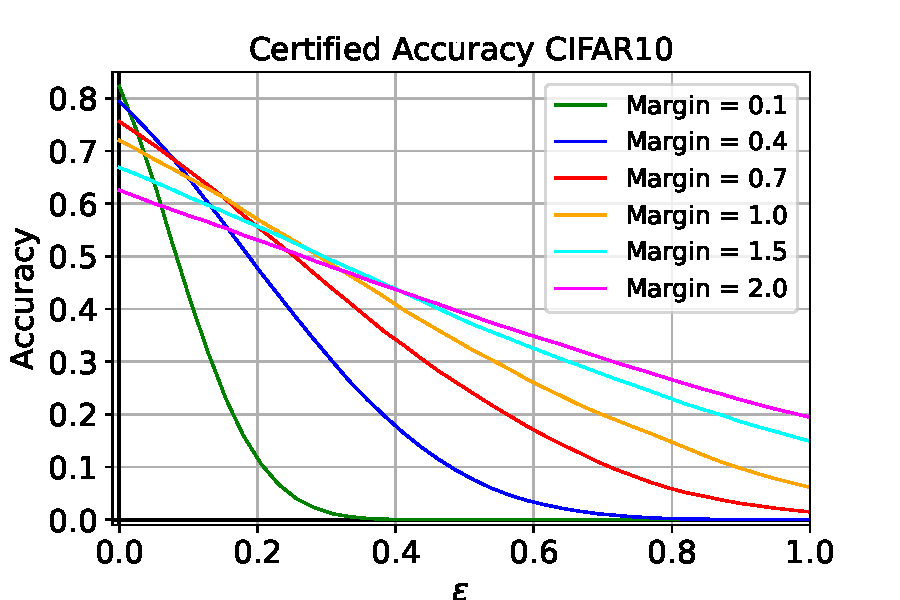
\includegraphics[width=0.48\textwidth]{sections/4_certification/images/cert_acc_margin_eps_c10.pdf}&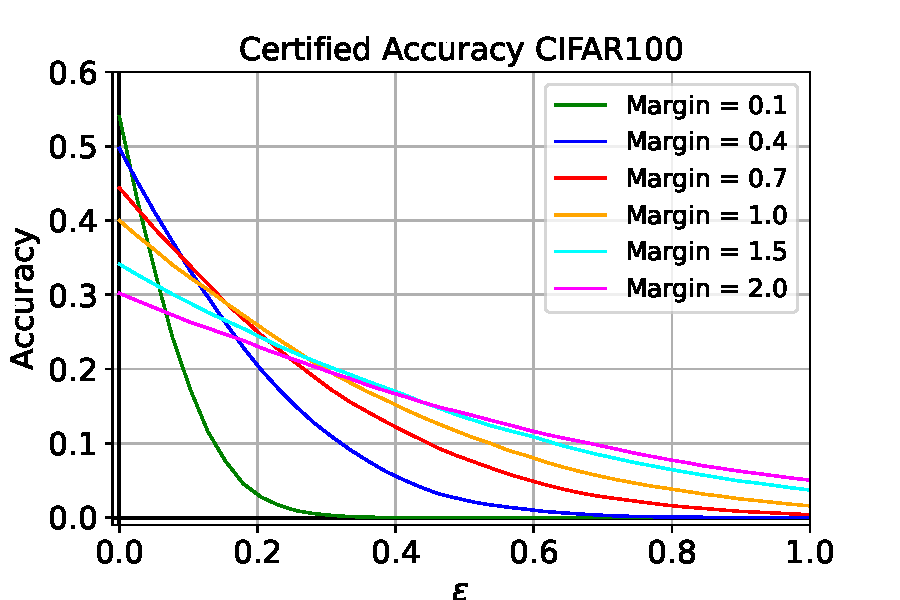
\includegraphics[width=0.48\textwidth]{sections/4_certification/images/cert_acc_margin_eps_c100.pdf}
    \end{tabular}
    \caption{Certifiably robust accuracy w.r.t. the perturbation $\varepsilon$ for our CPL-S  network with different margin parameters on CIFAR10 and CIFAR100 datasets.}
    \label{fig:cert-acc-margin}
\end{figure}


\begin{figure}[h]
    \centering
    \begin{tabular}{cc}
    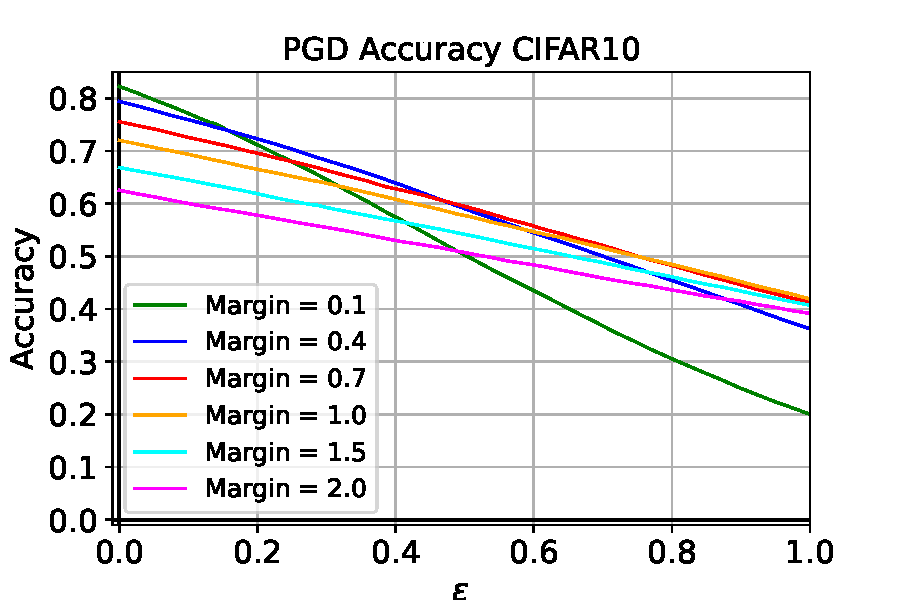
\includegraphics[width=0.49\textwidth]{sections/4_certification/images/pgd_acc_margin_eps_c10.pdf}&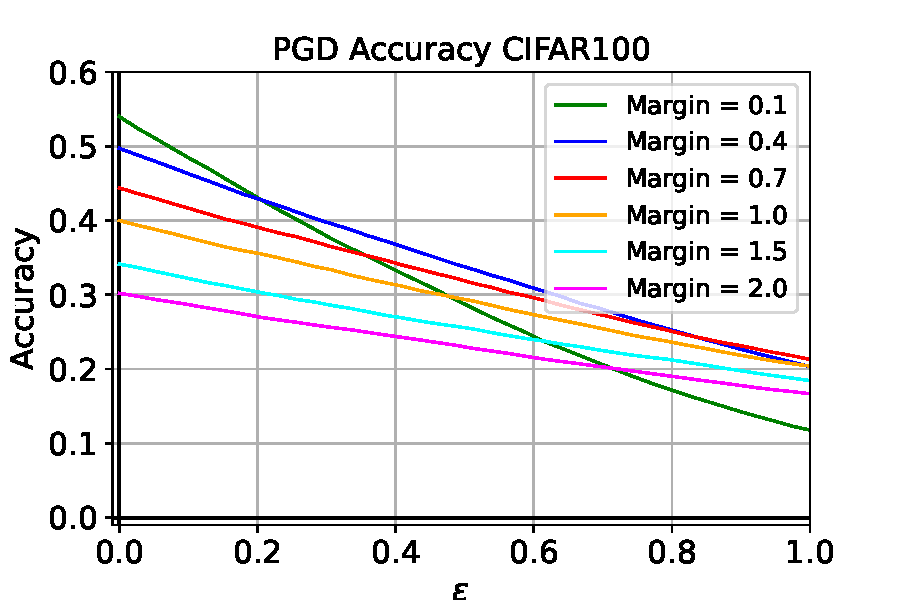
\includegraphics[width=0.49\textwidth]{sections/4_certification/images/pgd_acc_margin_eps_c100.pdf}
    \end{tabular}
    \caption{Certifiably robust accuracy w.r.t. the perturbation $\varepsilon$ for our CPL-S  network with different margin parameters on CIFAR10 and CIFAR100 datasets.}
    \label{fig:pgd-acc-margin}
\end{figure}

\paragraph{Effect of the Margin Parameter.}
In these experiments we varied the margin parameter in the margin loss in Figures~\ref{fig:cert-acc-margin} and~\ref{fig:pgd-acc-margin}. It clearly exhibits a tradeoff between standard and robust accuracy. When the margin is large, the standard accuracy is low, but the level of robustness remain high even for ``large'' perturbations. On the opposite, when the margin is small, we obtain a high standard accuracy but we are unable to keep a good robustness level as the perturbation increases. It is verified both on certified and empirical robustness.





\subsection{Training stability: scaling up to $1000$ layers}

\begin{figure}[h]
    \centering
    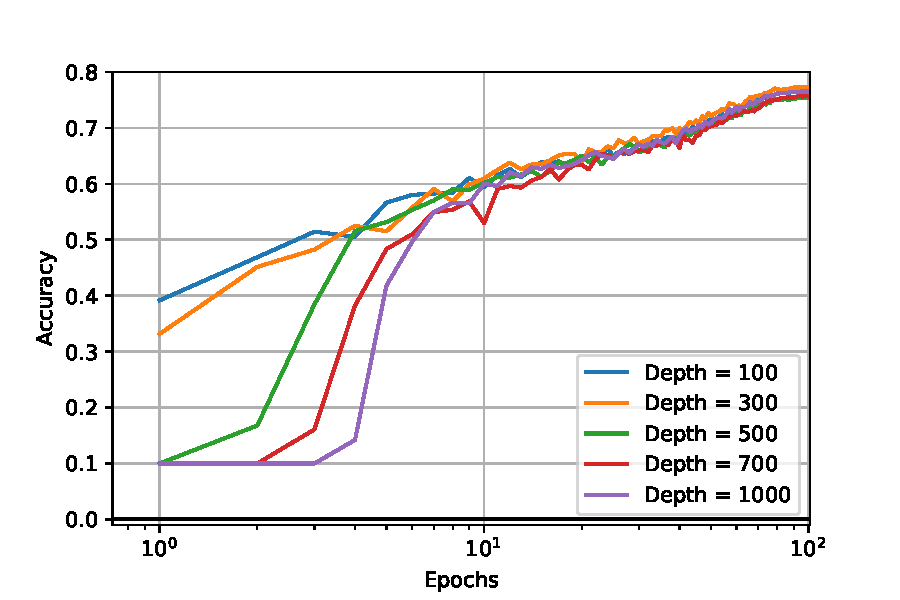
\includegraphics[width=0.5\textwidth]{sections/4_certification/images/final_cifar10_veryverydeep.pdf}
    \caption{Standard test accuracy w.r.t. the number of epochs (log-scale) for various depths for our neural networks ($100,300,500,700,1000$).}
    \label{fig:verydeep}
\end{figure}

While the Residual Network architecture limits, by design, gradient vanishing issues, it still suffers from exploding gradients in many cases~\citep{hayou2021stable}.
To prevent such scenarii, batch normalization layers~\citep{ioffe2015batch} are used in most Residual Networks to stabilize the training.

Recently, several works~\citep{miyato2018spectral,farnia2018generalizable} have proposed to normalize the linear transformation of each layer by their spectral norm.
Such a method would limit exploding gradients but would again suffer from gradient vanishing issues.
Indeed, spectral normalization might be too restrictive: dividing by the spectral norm can make other singular values vanishingly
small.
While more computationally expensive (spectral normalization can be done with $1$ Power Method iteration), orthogonal projections prevent both exploding and vanishing issues. 

On the contrary the architecture proposed  has the advantage to naturally control the gradient norm of the output with respect to a given layer.
Therefore, our architecture can get the best of both worlds: limiting exploding and vanishing issues while maintaining scalability. 
To demonstrate the scalability of our approach, we experiment the ability to scale our architecture to very high depth (up to 1000 layers) without any additional normalization/regularization tricks, such as Dropout~\citep{srivastava2014dropout}, Batch Normalization~\citep{ioffe2015batch} or gradient clipping~\citep{pascanu2013difficulty}.
With the work done by~\cite{xiao2018dynamical}, which leverage Dynamical Isometry and a Mean Field Theory to train a $10000$ layers neural network, we believe, to the best of our knowledge, to be the second to perform such training. 
For the sake of computation efficiency, we limit this experiment to architecture with $30$ feature maps.
We report the accuracy in terms of epochs for our architecture in Figure~\ref{fig:verydeep} for a varying number of convolutional layers.
It is worth noting that for the deepest networks, it may take a few epochs before the start of convergence.
As \cite{xiao2018dynamical}, we remark there is no gain in using very deep architecture for this task.


\subsection{Relaxing linear layers}

\begin{table*}
\begin{tabular}{lrrr}
\toprule
  & \multicolumn{1}{c}{\textbf{h = 1.0}} & \multicolumn{1}{c}{\textbf{h = 0.1}} & \multicolumn{1}{c}{\textbf{h = 0.01}} \\
\midrule
\textbf{Standard} & 85.10 & 82.23 & 78.53 \\
\textbf{PGD ($\varepsilon = 36/255$}) & 61.45 & 62.99 & 60.98 \\
\bottomrule
\end{tabular}
\caption{Level of accuracy of CPL networks when the constraints on the step-size is relaxed. We fixed the step-size $h$ to different values and measured standard and empirically robust accuracy. Here the CPL-M model is used.}
\label{table:relaxstep}
\end{table*}

Table~\ref{table:relaxstep} shows the result of the relaxed training of our CPL architecture, i.e. we fixed the step $h_t$ in the discretized convex potential flow of Proposition~\ref{prop:discrete_convex_potentials}.
Increasing the constant $h$ allows for an important improvement  in the standard accuracy, but we loose in robust empirical accuracy.
While computing the certified accuracy is not possible in this case due to the unknown value of the Lipschitz constant, we can still notice that the training of the network are still stable without normalization tricks, and offer a non-negligible level of robustness. 




\section{Discussions and Open questions}
In this chapter, we presented a new generic method to build $1$-Lipschitz layers.
We leverage the continuous time dynamical system interpretation of Residual Networks and show that using convex potential flows naturally defines $1$-Lipschitz neural networks.
After proposing a parametrization based on Input Convex Neural Networks~\citep{amos2017input}, we  show that our models  reach competitive results in classification and robustness in comparison which other existing $1$-Lipschitz approaches.
We also experimentally show that our layers provide scalable approaches without further regularization tricks to train very deep architectures.

Exploiting the ResNet architecture for devising flows have been an important research topic.
For example, in the context of generative modeling, Invertible Neural Networks~\citep{behrmann2019invertible} and Normalizing Flows~\citep{rezende2015variational, verine2021expressivity} are both import research topic.
More recently, Sylvester Normalizing Flows~\citep{vdberg2018sylvester} or Convex Potential Flows~\citep{huang2021convex} have had similar ideas to this present work but for a very different setting and applications. In particular, they did not have interest in the contraction property of convex flows and the link with adversarial robustness have been under-exploited.

% \paragraph{Exploiting other discretization schemes.} 
% Propoisition~\ref{prop:continuous-lip} gives a general argument to build $1$-Lipschitz Networks. We exploited some discretization schemes to build $1$-Lipschitz layers. One can imagine exploiting other  more complex discretization schemes as the implicit schemes, leap frog schemes. 

\paragraph{Expressivity of discretized convex potential flows.}
Propoisition~\ref{prop:continuous-lip} suggests to constraint the symmetric part of the Jacobian of $F_t$. We proposed to decompose $F_t$ as a sum of potential gradient and skew symmetric matrix. Finding other parametrizations is an open challenge.
Our models may not express all $1$-Lipschitz functions.
Knowing which functions can be approximated by our CPL layers is difficult even in the linear case. Indeed, let us define $\mathcal{S}_1(\RR^{d\times d})$ the space of real symmetric matrices with singular values bounded by $1$. Let us also define $\mathcal{M}_1(\RR^{d\times d})$ the space of real matrices with singular values bounded by $1$ in absolute value.
Let $\mathcal{P}(\RR^{d\times d})=\{A\in\RR^{d\times d}|\exists n\in \mathbb{N},S_1,\dots,S_n\in \mathcal{S}_1(\RR^d\times d)\text{ s.t. } A = S_1\dots S_n\}$. Then one can prove\footnote{A proof and justification of this result can be found \href{https://mathoverflow.net/questions/60174/factorization-of-a-real-matrix-into-hermitian-x-hermitian-is-it-stable}{here}.} that $\mathcal{P}(\RR^{d\times d}) \neq \mathcal{M}_1(\RR^{d\times d})$. Thus there exists $A\in\mathcal{M}_1(\RR^{d\times d})$ such that for all matrices $n$, for all matrices $S_1,\dots,S_n\in\mathcal{S}_1(\RR^{d\times d})$ such that $M\neq S_1,\dots,S_n$. Applied to the expressivity of discretized convex potential flows, the previous result means that there exists a $1$-Lipschitz linear function that cannot be approximated as a discretized flow of any depth of convex linear $1$-smooth potential flows as in Proposition~\ref{prop:discrete_convex_potentials}. Indeed such a flow would write: $x\mapsto\prod_i(1-2S_i)x$ where $S_i$ are symmetric matrices whose eigenvalues are in $[0,1]$, in other words such transformations are exactly described by $x\mapsto Mx$  for some $M\in\mathcal{P}(\RR^{d\times d})$. This is  an important question that requires further investigation. 


\paragraph{Going beyond ResNets} One can also think of extending  our work by the study of  other dynamical systems. Recent architectures such as Hamiltonian Networks~\citep{greydanus2019hamiltonian} and Momentum Networks~\citep{sander2021momentum} exhibit interesting properties and it worth digging into these architectures to build Lipschitz layers.
Finally, we hope to use similar approaches to build robust Recurrent Neural Networks~\citep{sherstinsky2020fundamentals} and Transformers~\citep{vaswani2017attention}. For Transformers,~\citet{vuckovic2020mathematical,sander2021sinkformers} has proposed a dynamical system interpretation of a flow on particles (i.e. the words in the the initial sentence). This can be seen as an interacting flow over a distributions. The question of robustness and Lipschitzness is way more technical since it implies Lipshitzness in the space of a distribution. One could imagine to use optimal transport~\citep{villani2003topics} and Wasserstein Gradient flows~\citep{ambrosio2005gradient} as tools for deriving Lipschitz guarantees for Transformers.









% \section{Proofs}

% \subsection{Proof of Proposition~\ref{prop:continuous-lip}}
% \label{proof:continuous-lip}

% \begin{proof}
% Consider the time derivative of the square difference between the two flows $x_t$ and $z_t$ associated with the function $F_t$ and following the definition~\ref{def:flow}: 
% \begin{align*}
%   \frac{d}{dt} \lVert x_t-z_t\rVert_2^2 & = 2 \big\langle x_t-z_t,\frac{d}{dt}( x_t-z_t)\big\rangle\\
%     &=2 \big\langle x_t-z_t,F_{\theta_{t}}(x_{t})-F_{\theta_{t}}(z_{t})\big\rangle \\
%     &=  2 \big\langle x_t-z_t,\int_0^1\nabla_xF_{\theta_{t}}(x_{t}+s(z_t-z_t))(x_t-z_t)ds\big\rangle\textrm{, by Taylor-Lagrange formula}\\ 
%     &=  2 \int_0^1\big\langle x_t-z_t,\nabla_xF_{\theta_{t}}(x_{t}+s(z_t-z_t))(x_t-z_t)\big\rangle ds\\
%      &=  2 \int_0^1\big\langle x_t-z_t,S(\nabla_xF_{\theta_{t}}(x_{t}+s(z_t-z_t)))(x_t-z_t)\big\rangle ds
% \end{align*}
% In the last step, we used that for every skew-symmetric matrix $A$ and vector $x$, $\lVert x,Ax\rVert = 0$.
% Since $\mu_tI\preceq S(\nabla_xF_{\theta_{t}}(x_{t}+s(z_t-y_t)))\preceq  \lambda_tI$, we get
% \begin{align*}
%  2\mu_t \lVert x_t-z_t\rVert_2^2 \leq \frac{d}{dt} \lVert x_t-z_t\rVert_2^2 \leq 2\lambda_t \lVert x_t-z_t\rVert_2^2
% \end{align*}
% Then by Gronwall Lemma, we have
% \begin{align*}
%   \lVert x_0-y_0 \rVert e^{\int_0^t\mu_s ds}\leq \lVert x_t-y_t \rVert\leq \lVert x_0-y_0 \rVert e^{ \int_0^t\lambda_s ds}
% \end{align*}
% which concludes the proof.
% \end{proof}

% \subsection{Proof of Corollary~\ref{cor:conv-skew}}
% \label{proof:conv-skew}
% \begin{proof}

% For all $t,x$, we have $F_t(x) = -\nabla_x f_{t}(x)+A_t x$ ~ so~
% $\nabla_x F_t(x) = -\nabla_x^2 f_{t}(x)+A_t$. Then $S(\nabla_x F_t(x)) =-\nabla_x^2 f_{t}(x)$. Since $f$ is convex, we have $\nabla_x^2 f_{t}(x)\succeq 0$. So by application of Proposition~\ref{prop:continuous-lip}, we deduce $\lVert x_t-y_t \rVert\leq \lVert x_0-y_0 \rVert$ for all trajectories starting from $x_0$ and $y_0$.
% \end{proof}

% \subsection{Proof of Proposition~\ref{prop:discrete_convex_potentials}}
% \label{proof:discrete_convex_potentials}
% \begin{proof}
% With $c_t = \lVert x_t -z_t\rVert_2^2$, we can write:
% \begin{align*}
%    c_{t+\frac12} - c_t = &-2 h_t \big\langle x_t - z_t, \nabla_xF_{\theta_{t}}(x_t) - \nabla_xF_{\theta_{t}}(z_t)  \big\rangle+ h_t^2 \lVert \nabla_xF_{\theta_{t}}(z_t) - \nabla_xF_{\theta_{t}}(z_t)\rVert_2^2
% \end{align*}
% This equality allows us to derive the equivalence between  $c_{t+1} \leq c_t$ and: 
% \begin{align*}
%    \frac{h_t}{2}
%    \lVert  \nabla F_{\theta_{t}}(x_t) - \nabla F_{\theta_{t}}(z_t)\rVert_2^2
%    \leq
%    \langle x_t -z_t, \nabla F_{\theta_{t}}(z_t) - \nabla F_{\theta_{t}}(z_t) \rangle 
% \end{align*}
% Moreover, assuming that $F_{\theta_t}$ being  that:
% \begin{align*}
%    \frac{1}{L_t} &\lVert \nabla_xF_{\theta_{t}}(x_t) - \nabla_xF_{\theta_{t}}(z_t)\rVert_2^2 
%    \leq\big\langle x_t -z_t, \nabla_xF_{\theta_{t}}(x_t) - \nabla_xF_{\theta_{t}}(z_t) \big\rangle
% \end{align*}
% We can see with this last inequality that if we enforce  $h_t \leq \frac{2}{L_t}$, we get $c_{t+\frac12} \leq c_t$ which concludes the proof.
% \end{proof}


% \section{Additional Results}

% % \subsection{Functions whose gradient is skew-symmetric everywhere}
% % \label{sup:skew}
% Let $F:=(F_1,\dots,F_d):\RR^d\to\RR^d$ be a twice differentiable function such that $\nabla F(x)$ is skew-symmetric for all $x\in\RR^d$. Then we have for all $i,j,k$:
% \begin{align*}
%     \partial_i\partial_j F_k =  -\partial_i\partial_k F_j =-\partial_k\partial_i F_j = \partial_k\partial_j F_i = \partial_j\partial_k F_i = -\partial_j\partial_i F_k = -\partial_i\partial_j F_k
% \end{align*}
% So we have $\partial_i\partial_j F_k =0$ and then $F$ is linear: there exists a skew-symmetric matrix $A$ such that $F(x)=Ax$ 


% \subsection{Implicit discrete convex potential flows}
% \label{sup:implicit}

% Let us define the implicit update $x_{t+\frac12} = x_{t}-\nabla_xf_{t}(x_{t+\frac12})$. Let us remark that $x_{t+\frac12}$ is uniquely defined as:
% \begin{align*}
%  x_{t+\frac12} =\argminB_{x\in\RR^d} \frac 12\lVert x-x_t\rVert^2+ f_t(x)  
% \end{align*}
% We recognized here the proximal operator of $f_t$ that is uniquely defined since $f_t$ is convex. Moreover we have for two trajectories $x_t$ and $z_t$:
% \begin{align*}
%    \lVert x_t-z_t\rVert^2_2& =  \lVert x_{t+\frac12}-z_{t+\frac12} +\nabla_xf_{t}(x_{t+\frac12})-\nabla_xf_{t}(z_{t+\frac12}) \rVert^2_2 \\
%    &=  \lVert x_{t+\frac12}-z_{t+\frac12}\rVert^2 + 2\langle x_t-z_t,\nabla_xf_{t}(x_{t+\frac12})-\nabla_xf_{t}(z_{t+\frac12})\rangle +\lVert\nabla_xf_{t}(x_{t+\frac12})-\nabla_xf_{t}(z_{t+\frac12}) \rVert^2_2 \\
%    &\geq  \lVert x_{t+\frac12}-z_{t+\frac12}\rVert^2 
% \end{align*}
% where the last inequality is deduced from the convexity of $f_t$. So, without any further assumption on $f_t$, the discretized implicit convex potential flow is $1$-Lipschitz.

% To compute such a layer, one could solve the proximal operator strongly convex-minimization optimization problem. This strategy is not computationally efficient and not scalable. 




% \subsection{Expressivity of discretized convex potential flows}
% \label{app:express}
% Let us define $\mathcal{S}_1(\RR^{d\times d})$ the space of real symmetric matrices with singular values bounded by $1$. Let us also define $\mathcal{M}_1(\RR^{d\times d})$ the space of real matrices with singular values bounded by $1$ in absolute value.
% Let $\mathcal{P}(\RR^{d\times d})=\{A\in\RR^{d\times d}|\exists n\in \mathbb{N},S_1,\dots,S_n\in \mathcal{S}_1(\RR^d\times d)\text{ s.t. } A = S_1\dots S_n\}$. Then one can prove\footnote{A proof and justification of this result can be found here: \url{https://mathoverflow.net/questions/60174/factorization-of-a-real-matrix-into-hermitian-x-hermitian-is-it-stable}} that $\mathcal{P}(\RR^{d\times d}) \neq \mathcal{M}_1(\RR^{d\times d})$. Thus there exists $A\in\mathcal{M}_1(\RR^{d\times d})$ such that for all matrices $n$, for all matrices $S_1,\dots,S_n\in\mathcal{S}_1(\RR^{d\times d})$ such that $M\neq S_1,\dots,S_n$. 

% Applied to the expressivity of discretized convex potential flows, the previous result means that there exists a $1$-Lipschitz linear function that cannot be approximated as a discretized flow of any depth of convex linear $1$-smooth potential flows as in Proposition~\ref{prop:discrete_convex_potentials}. Indeed such a flow would write: $x\mapsto\prod_i(1-2S_i)x$ where $S_i$ are symmetric matrices whose eigenvalues are in $[0,1]$, in other words such transformations are exactly described by $x\mapsto Mx$  for some $M\in\mathcal{P}(\RR^{d\times d})$.




\section{Additional experiments}
\label{app:xp-supp}

\subsection{Training stability: scaling up to $1000$ layers}

\begin{figure}[h]
    \centering
    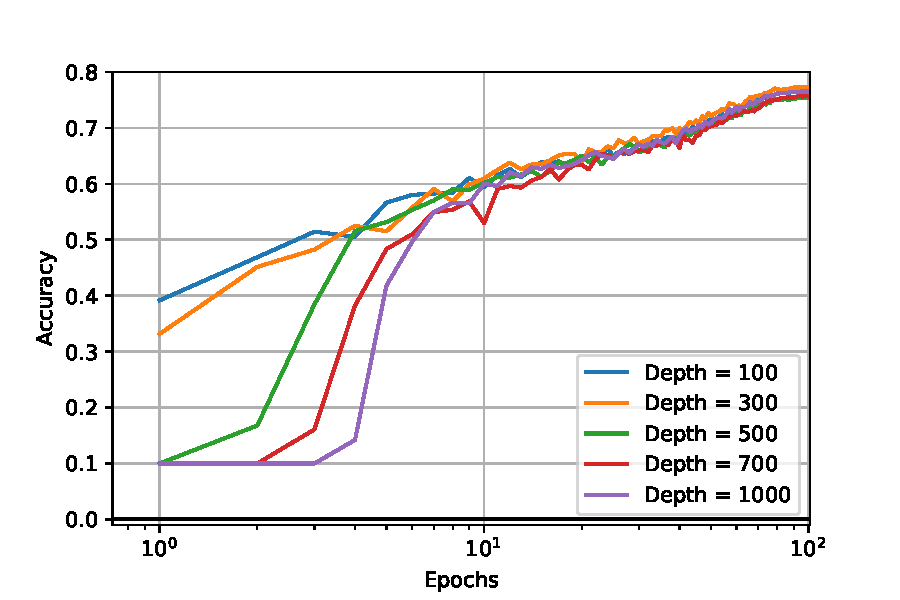
\includegraphics[width=0.5\textwidth]{sections/4_certification/images/final_cifar10_veryverydeep.pdf}
    \caption{Standard test accuracy in function of the number of epochs (log-scale) for various depths for our neural networks ($100,300,500,700,1000$).}
    \label{fig:verydeep}
\end{figure}

While the Residual Network architecture limits, by design, gradient vanishing issues, it still suffers from exploding gradients in many cases~\citep{hayou2021stable}.
To prevent such scenarii, batch normalization layers~\citep{ioffe2015batch} are used in most Residual Networks to stabilize the training.

Recently, several works~\citep{miyato2018spectral,farnia2018generalizable} have proposed to normalize the linear transformation of each layer by their spectral norm.
Such a method would limit exploding gradients but would again suffer from gradient vanishing issues.
Indeed, spectral normalization might be too restrictive: dividing by the spectral norm can make other singular values vanishingly
small.
While more computationally expensive (spectral normalization can be done with $1$ Power Method iteration), orthogonal projections prevent both exploding and vanishing issues. 

On the contrary the architecture proposed in this paper has the advantage to naturally control the gradient norm of the output with respect to a given layer.
Therefore, our architecture can get the best of both worlds: limiting exploding and vanishing issues while maintaining scalability. 
To demonstrate the scalability of our approach, we experiment the ability to scale our architecture to very high depth (up to 1000 layers) without any additional normalization/regularization tricks, such as Dropout~\citep{srivastava2014dropout}, Batch Normalization~\citep{ioffe2015batch} or gradient clipping~\citep{pascanu2013difficulty}.
With the work done by~\cite{xiao2018dynamical}, which leverage Dynamical Isometry and a Mean Field Theory to train a $10000$ layers neural network, we believe, to the best of our knowledge, to be the second to perform such training. 
For sake of computation efficiency, we limit this experiment to architecture with $30$ feature maps.
We report the accuracy in terms of epochs for our architecture in Figure~\ref{fig:verydeep} for a varying number of convolutional layers.
It is worth noting that for the deepest networks, it may take a few epochs before the start of convergence.
As \cite{xiao2018dynamical}, we remark there is no gain in using very deep architecture for this task.


\subsection{Relaxing linear layers}

\begin{center}
\begin{tabular}{lrrr}
\toprule
  & \multicolumn{1}{c}{\textbf{h = 1.0}} & \multicolumn{1}{c}{\textbf{h = 0.1}} & \multicolumn{1}{c}{\textbf{h = 0.01}} \\
\midrule
\textbf{Clean} & 85.10 & 82.23 & 78.53 \\
\textbf{PGD ($\varepsilon = 36/255$}) & 61.45 & 62.99 & 60.98 \\
\bottomrule
\end{tabular}%
\end{center}
The table above shows the result of the relaxed training of our StableBlock architecture, i.e. we fixed the step $h_t$ in the discretized convex potential flow of Proposition~\ref{prop:discrete_convex_potentials}.
Increasing the constant $h$ allows for an important improvement  in the clean accuracy, but we loose in robust empirical accuracy.
While computing the certified accuracy is not possible in this case due to the unknown value of the Lipschitz constant, we can still notice that the training of the network are still stable without normalization tricks, and offer a non-negligible level of robustness. 





\subsection{Effect of Batch Size in Training}


\begin{table*}[h]
  \centering
  \sisetup{%
    table-align-uncertainty=true,
    separate-uncertainty=true,
    detect-weight=true,
    detect-inline-weight=math
  }
  \begin{tabular}
  {
    l
    S[table-format=2.2]
    S[table-format=2.2]
    S[table-format=2.2]
    S[table-format=2.2]
    S[table-format=2.2]
    S[table-format=2.2]
  }
  \toprule
  &\multicolumn{1}{c}{\textbf{Batch size }}& \multicolumn{1}{c}{\textbf{Clean Accuracy}} & \multicolumn{3}{c}{\textbf{Provable Accuracy ($\varepsilon $)}} &  \multicolumn{1}{c}{\textbf{Time per epoch (s)}} 
    \\
    \cmidrule{4-6}
    & \multicolumn{1}{c}{ } & \multicolumn{1}{c}{ } &\multicolumn{1}{c}{36/255} & \multicolumn{1}{c}{72/255} &  \multicolumn{1}{c}{108/255} & \multicolumn{1}{c}{\textbf{}} 
    \\
  \midrule
    \multirow{3}{*}{\textbf{CPL-S}} & 64 & 76.5& 62.9 & 47.3 & 32.0 & 48 \\
                                    & 128 & 76.1 & 62.8 & 47.1 & 32.3  & 31 \\
                                    & 256 & 75.6 & 62.3 & 46.9 & 32.2 & 22 \\
    \midrule
 \multirow{3}{*}{\textbf{CPL-M}} & 64 & 77.4 & 63.6 & 47.4 & 32.1  & 77 \\
                                    & 128 & 77.2 &63.5 & 47.5 & 32.1 & 50 \\
                                    & 256 & 76.8 & 63.2 & 47.4 & 32.4& 40 \\
    \midrule

 \multirow{3}{*}{\textbf{CPL-L}} & 64 & 78.4 & 64.2 & 47.8 & 32.2  & 162 \\
                                    & 128 & 78.2 & 64.3 & 47.9 & 32.5 & 109 \\
                                    & 256 & 77.6 & 63.9 & 48.1 & 32.7& 93 \\
  \midrule
 \multirow{3}{*}{\textbf{CPL-XL}} & 64 & 78.9 & 64.2 & 47.2 & 31.2  & 271 \\
                                    & 128 & 78.9 & 64.2 & 47.5 & 31.8 & 198 \\
                                    & 256 &78.5 & 64.4 & 47.8 & 32.4& 163 \\

  \bottomrule
  \end{tabular}%
  \caption{Results on the CIFAR10 dataset on standard and  provably certifiable accuracies for different values of perturbations $\varepsilon$ on CPL (ours) models with various batch sizes. The average time per epoch in seconds is also reported in the last column. All the reported networks use Last Layer Normalization.}
  \label{table:c10-comp-bs}%
\end{table*}%



\begin{table*}[h]
  \centering
  \sisetup{%
    table-align-uncertainty=true,
    separate-uncertainty=true,
    detect-weight=true,
    detect-inline-weight=math
  }
  \begin{tabular}
  {
    l
    S[table-format=2.2]
    S[table-format=2.2]
    S[table-format=2.2]
    S[table-format=2.2]
    S[table-format=2.2]
    S[table-format=2.2]
  }
  \toprule
  &\multicolumn{1}{c}{\textbf{Batch size }}& \multicolumn{1}{c}{\textbf{Clean Acc.}} & \multicolumn{3}{c}{\textbf{Provable Acc. ($\varepsilon $)}} &  \multicolumn{1}{c}{\textbf{Time per epoch (s)}} 
    \\
    \cmidrule{4-6}
    & \multicolumn{1}{c}{ } & \multicolumn{1}{c}{ } &\multicolumn{1}{c}{36/255} & \multicolumn{1}{c}{72/255} &  \multicolumn{1}{c}{108/255} & \multicolumn{1}{c}{\textbf{}} 
    \\
  \midrule
  \multirow{3}{*}{\textbf{CPL-S}} & 64 & 45,6 & 30,8 & 19,3 & 11,2 & 47 \\
                                    & 128 & 44,9 & 30,7 & 19,2 & 11,0 & 31\\
                                    & 256 & 44,0 & 29,9 & 19,1 & 10,9 & 23\\
  \midrule
  \multirow{3}{*}{\textbf{CPL-M}} & 64 & 46.6 & 31,6 & 19,6 & 11,6 & 78 \\
                                    & 128 & 46.3 & 31,1 & 19,7 & 11,5 & 55 \\
                                    & 256 & 45.6 & 31,1 & 19,3 & 11,3 & 41 \\

  \midrule

  \multirow{3}{*}{\textbf{CPL-L}} & 64 & 48.1 & 32,7 & 20,3 & 11,7 & 163 \\ 
                                    & 128 & 47,4 & 32,3 & 20,0 & 11,8 & 116 \\ 
                                    & 256 & 46,8 & 31,8 & 20,1 & 11,7 & 95 \\ 
  \midrule
  \multirow{3}{*}{\textbf{CPL-XL}} & 64 & 49,0 & 33,7 & 21,1 & 12,0 & 293 \\
                                    & 128 & 48,0 & 33,7 & 21,0 & 12,1 & 209 \\
                                    & 256 &47,8 & 33,4 & 20,9 & 12,6 & 164 \\

  \bottomrule
  \end{tabular}%
  \caption{Results on the CIFAR100 dataset on standard and  provably certifiable accuracies for different values of perturbations $\varepsilon$ on CPL (ours) models with various batch sizes. The average time per epoch in seconds is also reported in the last column. All the reported networks use Last Layer Normalization.}
  \label{table:c100-comp-bs}%
\end{table*}%

In Tables~\ref{table:c10-comp-bs} and~\ref{table:c100-comp-bs}, we tried three different batch sizes (64, 128 and 256) for training our networks on CIFAR10 and CIFAR100 datasets, we remark a gain in standard accuracy in reducing the batch size for all settings. As the perturbation becomes larger, the gain in accuracy is reduced and can even in some cases we may loose some points in robustness.

\subsection{Effect of the Margin Parameter}

\begin{figure}[h]
    \centering
    \begin{tabular}{cc}
    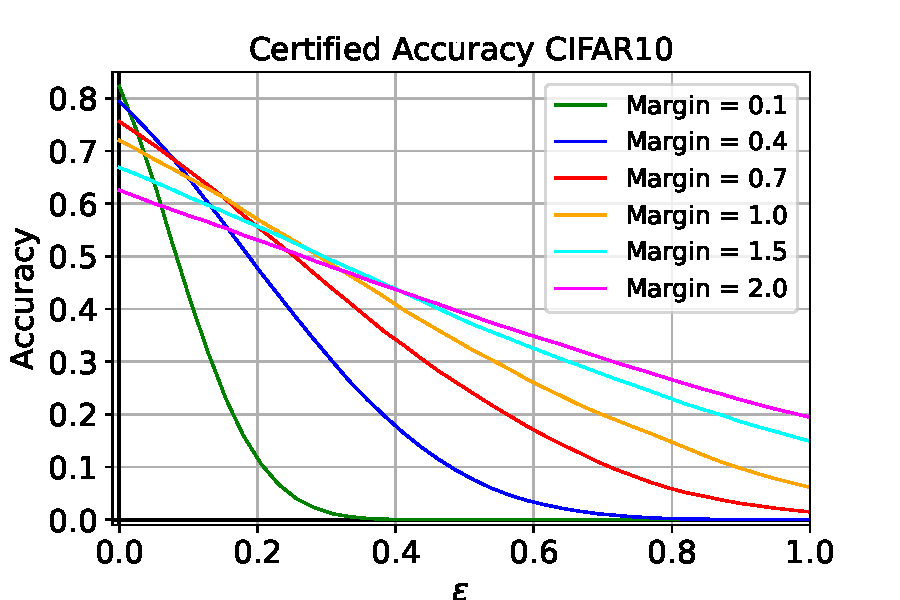
\includegraphics[width=0.49\textwidth]{sections/4_certification/images/cert_acc_margin_eps_c10.pdf}&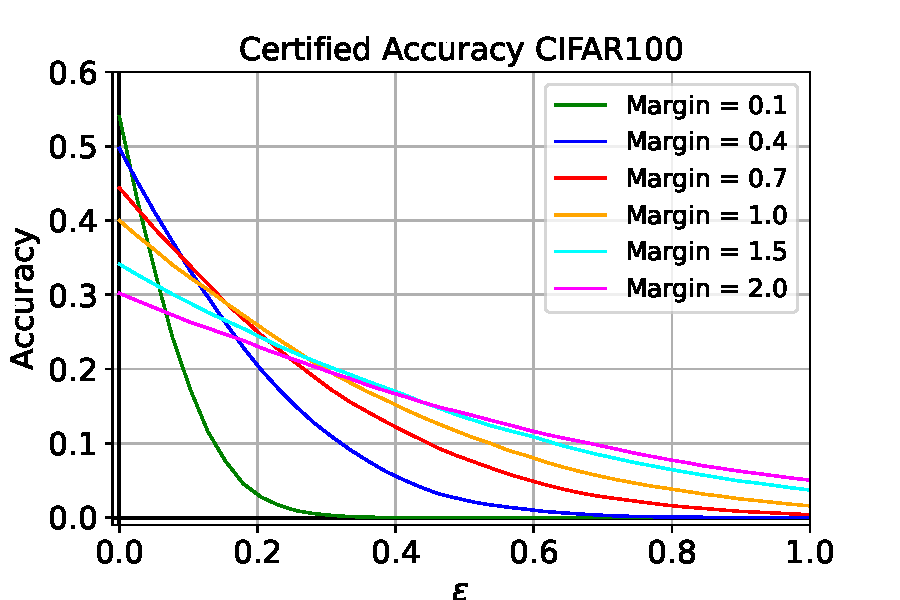
\includegraphics[width=0.49\textwidth]{sections/4_certification/images/cert_acc_margin_eps_c100.pdf}
    \end{tabular}
    \caption{Certifiably robust accuracy in function of the perturbation $\varepsilon$ for our CPL-S  network with different margin parameters on CIFAR10 and CIFAR100 datasets.}
    \label{fig:cert-acc-margin}
\end{figure}


\begin{figure}[h]
    \centering
    \begin{tabular}{cc}
    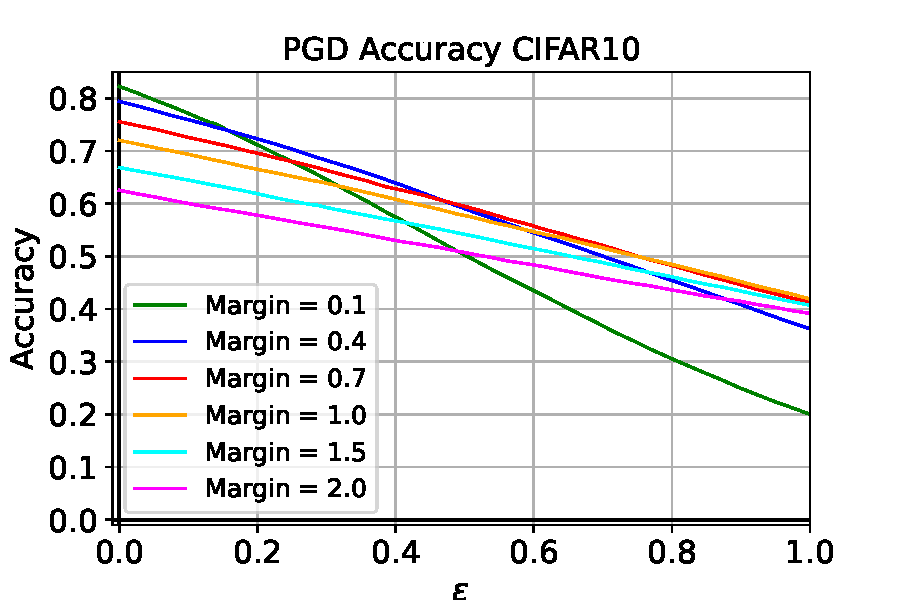
\includegraphics[width=0.49\textwidth]{sections/4_certification/images/pgd_acc_margin_eps_c10.pdf}&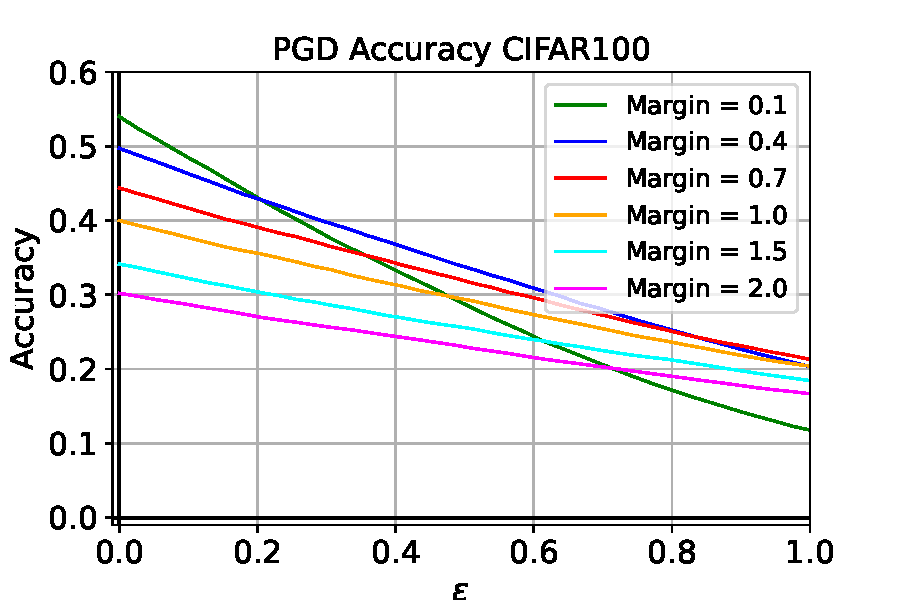
\includegraphics[width=0.49\textwidth]{sections/4_certification/images/pgd_acc_margin_eps_c100.pdf}
    \end{tabular}
    \caption{Certifiably robust accuracy in function of the perturbation $\varepsilon$ for our CPL-S  network with different margin parameters on CIFAR10 and CIFAR100 datasets.}
    \label{fig:pgd-acc-margin}
\end{figure}

In these experiments we varied the margin parameter in the margin loss in Figures~\ref{fig:cert-acc-margin} and~\ref{fig:pgd-acc-margin}. It clearly exhibits a tradeoff between standard and robust accuracy. When the margin is large, the standard accuracy is low, but the level of robustness remain high even for ``large'' perturbations. On the opposite, when the margin is small, we get a high standard accuracy but we are unable to keep a good robustness level as the perturbation increases. It is verified both on certified and empirical robustness.



